%% -----------------------------------------------------------------
%% This file uses UTF-8 encoding
%%
%% For compilation use following command:
%% latexmk -pdf -pvc -bibtex thesis
%%
%% -----------------------------------------------------------------
%%                                     _     _      
%%      _ __  _ __ ___  __ _ _ __ ___ | |__ | | ___ 
%%     | '_ \| '__/ _ \/ _` | '_ ` _ \| '_ \| |/ _ \
%%     | |_) | | |  __/ (_| | | | | | | |_) | |  __/
%%     | .__/|_|  \___|\__,_|_| |_| |_|_.__/|_|\___|
%%     |_|                                          
%%
%% -----------------------------------------------------------------

\documentclass{kithesis}
\usepackage{hyperref}
\usepackage{glossaries}
\usepackage{array}
% Additional packages
\usepackage[main=slovak,english]{babel}
% For thesis written in English just change the order of languages:
% \usepackage[main=english,slovak]{babel}

\usepackage{listings}  % for source code
% Listings settings
% See for details: https://en.wikibooks.org/wiki/LaTeX/Source_Code_Listings
\lstset{
    basicstyle=\small\ttfamily,  % smaller typewriter font
    showstringspaces=false       % don't show spaces in string
}

% Location of file with bibliography resources
\addbibresource{chapters/bibliography.bib}

% Variables
\thesisspec{figures/zadavaci-list.png} 

\title{My thesis \br (the skeleton)}{IoT projekt pre stredné školy II \br }

\author{Denys}{Lashuk}
\supervisor{Miroslav Biňas} %veduci prace
%\consultant{Donald E. Knuth} %konzultant
%\college{University of Žilina}{Žilinská univerzita} %univerzita
%\faculty{Faculty of Electrical Engineering and informatics}{Fakulta elektrotechniky a informatiky} %fakulta
%\department{Department of Computers and Informatics}{Katedra počítačov a informatiky} %katedra
%\departmentacr{DCI}{KPI} % skratka katedry
%\thesis{Master thesis}{Diplomová práca} %typ prace
\submissiondate{13}{5}{2023}
%\fieldofstudy{9.2.1 Informatika}
%\studyprogramme{Informatika}
%\city{Košice} %mesto
\keywords{\LaTeX, programming, typesetting}{\LaTeX, programovanie, sadzba textu}
%\declaration{som nepodvadzal}

\abstract{%
    % english 
	\blindtext
}{%
    % slovak 
	\blindtext
}

\acknowledgment{Na tomto mieste by som rád poďakoval svojmu vedúcemu práce Miroslavu Biňasu za jeho čas a odborné vedenie počas riešenia mojej práce.

Chcem poďakovať všetkým svojim blízkym a priateľom, ktorí ma podporovali. iež by som chcel poďakovať chatu GPT a prekladateľovi DeepL za pomoc pri písaní tejto práce.
}
% if you want to work only on selected chapters
%\includeonly{chapters/analyza} %,chapters/synteza}

% Load acronyms
% Acronyms
% ========
%
% An acronym is a word formed from the initial letters in a phrase. 
%
% Acronym Definition Exapmle:
% ---------------------------
% \newacronym{gcd}{GCD}{Greatest Common Divisor}
% \newacronym{dry}{DRY}{Don't Repeat Yourself}
%
% Usage:
% ------
% You can use these three options:
% 
% \acrlong{}  
%   Displays the phrase which the acronyms stands for. Put the label of the acronym inside the braces. In the example, \acrlong{gcd} prints Greatest Common Divisor. 
%
% \acrshort{} 
%   Prints the acronym whose label is passed as parameter. For instance, \acrshort{gcd} renders as GCD. 
%
% \acrfull{ } 
%   Prints both, the acronym and its definition. In the example the output of \acrfull{dry} is Don't Repeat Yourself (DRY). 
% 
% For more information see:
% -------------------------
% * https://www.sharelatex.com/learn/Glossaries 
% * https://en.wikibooks.org/wiki/LaTeX/Glossary
%


\newacronym{gcd}{GCD}{Greatest Common Divisor}
\newacronym{lcm}{LCM}{Least Common Multiple}



%% -----------------------------------------------------------------
%%          _                                       _   
%%       __| | ___   ___ _   _ _ __ ___   ___ _ __ | |_ 
%%      / _` |/ _ \ / __| | | | '_ ` _ \ / _ \ '_ \| __|
%%     | (_| | (_) | (__| |_| | | | | | |  __/ | | | |_ 
%%      \__,_|\___/ \___|\__,_|_| |_| |_|\___|_| |_|\__|
%%                                                      
%% -----------------------------------------------------------------

\begin{document}
%% Title page, abstract, declaration etc.:
\frontmatter{}

%% List of code listings, if you are using package minted
%\listoflistings

%\pagenumbering{arabic}

%% Chapters
% !TEX root = ../thesis.tex

\chaptermark{Úvod}
\phantomsection
\addcontentsline{toc}{chapter}{Úvod}

\chapter*{Úvod}

V dnešnom svete, kde technológie sú centrom nášho každodenného života, je rozvoj internetu vecí čoraz dôležitejší. Internet vecí otvára veľké možnosti komunikácie medzi zariadeniami a predmetmi okolo nás a má veľký potenciál ovplyvňovať na rôzne oblasti nášho života vrátane školstva. Preto je podpora internetu vecí v školách mimoriadne dôležitá. Zamyslime sa nad tým, aký význam má implementácia internetu vecí do vyučovacieho procesu a aké sú jeho výhody pre študentov a učiteľov.

Implementácia IoT do školského vyučovania dáva študentom možnosť rozvíjať schopnosti, ktoré budú potrebovať v budúcnosti. Prostredníctvom internetu vecí sa žiaci môžu naučiť pracovať so senzormi, sieťami, aktuátormi a inými zariadeniami, ktoré si vyžadujú programátorské schopnosti a pochopenie technológií. Tým sa rozvíja ich kreativita, schopnosť riešiť problémy a tímová práca.

Podpora internetu vecí v školách pomáha zvyšovať záujem študentov o vedu a techniku. Vďaka IoT môžu žiaci vidieť konkrétne príklady použitia technológií v reálnom svete. Môžu vytvárať projekty, ktoré si vyžadujú pochopenie fyziky, matematiky, programovania a ďalších predmetov. To im pomáha pochopiť prepojenie medzi teoretickým učením a praktickým využitím vedomostí.

Implementácia internetu vecí do školského vzdelávania môže výrazne zlepšiť učenie a rozvoj žiakov. Okrem toho je podpora internetu vecí v školách dôležitá aj pre rozvoj technologickej gramotnosti učiteľov. Učitelia musia byť dobre oboznámení s novými technológiami, aby ich mohli efektívne využívať v školských hodinách. Získanie zručností v oblasti internetu vecí umožní učiteľom používať inovatívne vyučovacie metódy, zapojiť žiakov do aktívnej účasti a vytvoriť dynamické vzdelávacie prostredie.

Implementácia internetu vecí do škôl má veľký význam. Pomáha rozvíjať zručnosti budúcnosti, zvyšovať záujem študentov o vedu a technológie, zlepšovať učenie a rozvoj žiakov a rozvíjať technologickú gramotnosť učiteľov. Školy by mali aktívne podporovať internet vecí a začleniť ho do vzdelávacieho procesu, aby pripravili mladú generáciu na život v modernom technologickom svete.

\section*{Formulácia úlohy}
Mojím cieľom je vytvoriť projekt internetu vecí, ktorý by sa dal jednoducho implementovať do kurzu pre stredné školy na Slovensku, počas ktorého by sa študenti oboznámili so základmi internetu vecí. 

Preto som si v rámci tejto bakalárskej práce stanovil cieľ:
\begin{enumerate}
    \item Vytvoriť projekt internetu vecí, ktorý je zameraný na vzdelávací stupeň študentov stredných škôl a obsahuje aspoň základné funkcie štandardného produktu internetu vecí.
    \item Zamyslieť sa nad tým, ako budú študenti tento projekt vyvíjať a vytvoriť kostru projektu, ktorá by tento vývoj uľahčila.
    \item Otestujte svoj projekt na cieľovom publiku projektu a v prípade potreby vykonajte úpravy konečného riešenia.
    \item Odhadnúť cenu projektu.
    \item Vytvorť kvalitnú dokumentáciu projektu, aby ho učiteľ mohol ľahko implementovať do svojho kurzu.
\end{enumerate}
% !TEX root = ../thesis.tex

\chapter{Analytická časť}

%%---------------------------------------------------------------
\section{Čo je to Internet vecí}
Skôr ako začnete navrhovať a plánovať projekt internetu vecí, musíte najprv pochopiť definíciu internetu vecí a jeho základné princípy.

Takže, čo je to internet vecí? Ak sa spoľahneme na málo spoľahlivý zdroj, konkrétne na Wikipédiu, nájdeme nasledujúcu definíciu:

\textit{Internet vecí (\gls{iot}) označuje fyzické objekty (alebo skupiny takýchto objektov) so senzormi, spracovateľskými schopnosťami, softvérom a ďalšími technológiami, ktoré sa spájajú a vymieňajú si údaje s inými zariadeniami a systémami prostredníctvom internetu alebo iných komunikačných sietí.}\cite{wiki}

Môžem povedať, že táto definícia celkom dobre vystihuje základnú myšlienku tohto pojmu, ale myslím si, že jej chýba konkrétnosť. Čo sa týka akademickej definície internetu vecí, v tejto oblasti neexistuje vedecký konsenzus. Vo všeobecnosti si rôzni akademici definíciu mierne upravujú po svojom, ale ak to zhrnieme, najlepšia definícia by bola takáto:

\textit{An open and comprehensive network of intelligent objects that have the capacity to auto-organize, share information, data and resources, reacting and acting in face of situations and changes in the environment.}\cite{book}

Ďalším dôležitým aspektom porozumenia \gls{iot} je to, že je to sieť inteligentných zariadení, ktoré si vymieňajú dáta a táto sieť má svoju hierarchiu a logiku. To znamená, že jedno chytre zariadenie, aj keď má nejaký softvér a vykonáva konkrétnu úlohu (napríklad smartphone), nie je \gls{iot}, kým ho nepripojíte k sieti a nedáte mu konkrétnu úlohu v tejto sieti. Ako som už písal, sieť má svoju hierarchiu, ale pre štandardizáciu a koordináciu rôznych vývojov musí byť premyslená na základe nejakej architekturnej konceptuálnej modely. Napríklad v sieti Internet sú také konceptuálne modely, ako \textit{OSI} a \textit{TCP/IP}. V rámci \gls{iot} je tiež podobná architekturna model. Pokiaľ ide o vzhľad tejto modely, vedecká spoločnosť opäť nemá konsenzus. Na internete nájdete veľa rôznych architektúr s rôznymi počtami vrstiev a názvami, ale všetky majú približne rovnaký význam. V ďalšej práci budem používať architektonický model, ktorý sa skladá zo štyroch vrstiev.

\begin{figure}[!ht]
    \centering
    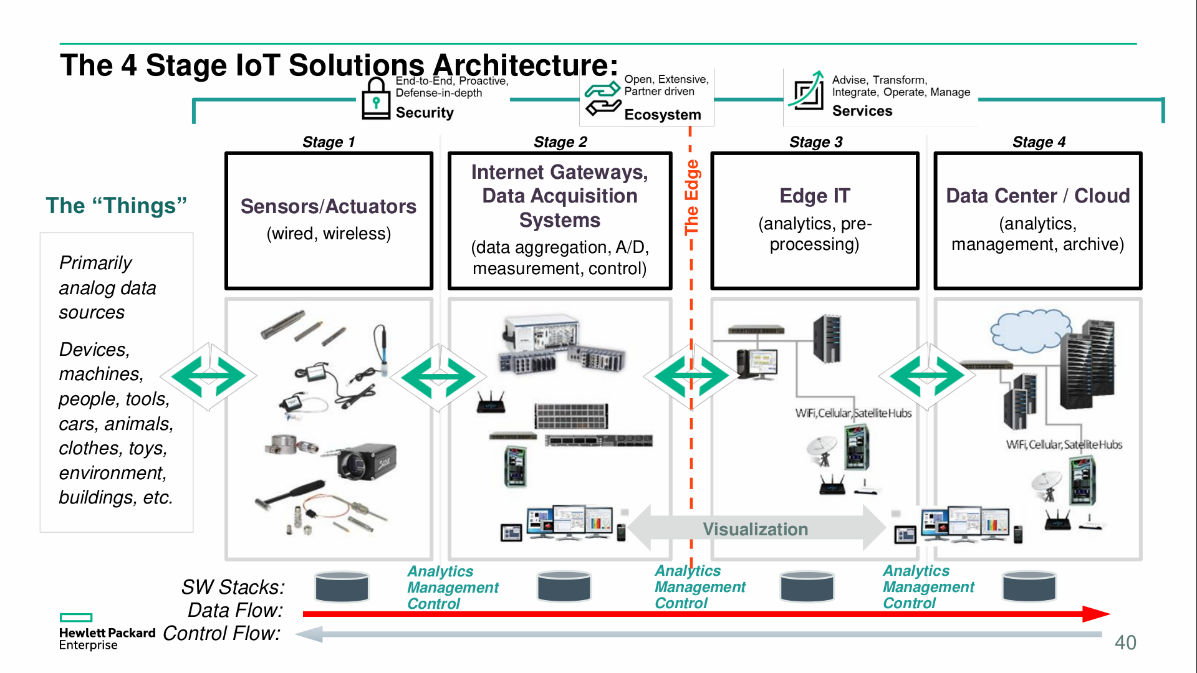
\includegraphics[width=.9\textwidth]{figures/iot}
    \caption{Vrstvy architektúry \gls{iot} riešení \label{iot} \cite{iotTukeLekcia1}}
\end{figure}

Zoznam jednotlivých vrstiev tohto modelu (obr. \ref{iot}) je nasledový:

\begin{itemize}
    \item \textit{Prvá vrstva}: Táto vrstva obsahuje snímače údajov a rôzne elektrické pohony na interakciu s prostredím. Môžu komunikovať s vyššou vrstvou aj medzi sebou. Objekty na tejto vrstve nemusia byť \textit{inteligentné} (napríklad DHT 11, motorček, mikrokontrolér).
    \item \textit{Druhá vrstva}: Na tejto vrstve sa nachádzajú brány prepojenia systému. Teda zariadenia, ktoré prijímajú údaje z predchádzajúcej vrstvy, poskytujú príkazy pohonov, vykonávajú primárne spracovanie a filtrovanie údajov a majú softvér. Táto úroveň sa zvyčajne fyzicky nachádza veľmi blízko k prvej a je jednou z najdôležitejších úrovní v celej sústave. Na tejto vrstve môže byť aj vizualizácia zozbieraných údajov.
    \item \textit{Tretia vrstva}: Táto vrstva slúži na zber a spracovanie údajov z predchádzajúcej vrstvy a ich pripravenie pre archiváciu alebo pre konečného spotrebiteľa. Zvyčajne táto úroveň slúži na zmiernenie zaťaženia hlavných serverov a na rýchlejšiu odpoveď používateľovi, ale môžu byť výnimky. Tretia vrstva nie je povinná pre použitie v \gls{iot} architektúre.
    \item \textit{Štvrtá vrstva}: Je konečnou vrstvou, na ktorej sa informácie analyzujú, archivujú alebo sa dostanú ku konečnému používateľovi používanie aplikácií.
\end{itemize}

Vychádzajúc z celého vyššie uvedeného, možno povedať, že koncept \gls{iot} a jeho architektúra riešia otázky zberu, spracovania a transportovania dát. Preto pri navrhovaní \gls{iot} riešení treba sústrediť pozornosť práve na správne manipulovanie s dátami.

V svojej prace sa budem snažiť dôsledne predstaviť študentom podstatu teoretického konceptu \gls{iot} a detailne ukázať všetky úrovne architektúry \gls{iot} riešení na príkladoch z praxe.

%%---------------------------------------------------------------

\section{Moje skúsenosti s vyučovaním \gls{iot} a prácou s elektronikou}
V tejto práci sa budem často rozhodovať na základe svojich skúseností, preto si myslím, že pred začatím samotnej analýzy a plánovania je potrebné sa podrobnejšie pozrieť na moje skúsenosti so vzdelávaním v oblasti \gls{iot}. Moje zoznámenie s \gls{iot} sa stalo až nedávno, v treťom ročníku môjho štúdia na univerzite v rámci predmetu \gls{iot}\cite{iotTuke}. Materiál tohto predmetu umožňuje rozšíriť znalosti v oblasti \gls{iot}, zoznámiť sa s jej rôznymi aspektmi, aby sme na konci semestra mohli navrhnúť a vytvoriť produkt na základe tejto koncepcie. Cieľom tohto kurzu je poskytnúť základné znalosti na úrovni junior developera v tejto oblasti. Celkovo som s týmto kurzom spokojný, ale chcem zdôrazniť jeho hlavnú nevýhodu, a to nevyváženosť praktických cvičení. Podľa môjho názoru boli praktické cvičenia viac zamerané na interakciu so systémom \textit{Docker} a menej na prácu s hardvérom. Okrem toho bolo učenie sa práce s hardvérom umiestnené až na konci a to tiež nie je podľa mňa najlepšia myšlienka.

Považujem, že základom \gls{iot} je interakcia s mikrokontrolérmi a mikroprocesormi, preto sa budem snažiť venovať väčšinu praktických úloh práve tejto interakcii. Je možné poznamenať, že \gls{iot} je koncept, ktorý sa stavia na komunikácii, nie na hardvéri.

Chcel by som spomenúť zaujímavú skúsenosť z účasti na workshopu zameranom na zoznámenie sa s \textit{ESP32}. Táto skúsenosť bola veľmi zaujímavá, pretože štruktúra prezentácie na tomto podujatí je tou, ktorú chcem zrealizovať aj vo svojom projekte. Teda, samotný webinár bol postavený takým spôsobom, že po krátkej teoretickej časti nasledovala praktická časť, čo umožňovalo udržiavať pozornosť poslucháčov neustále v strehu. V takomto vzdelávacom prístupe môžem identifikovať iba jednu nevýhodu - problém zaostávajúceho účastníka. Ak študent nestíha doháňať ostatných aspoň na jednej úrovni, bude pre neho veľmi ťažké udržiavať krok s ostatným materiálom.

%%---------------------------------------------------------------
\section{Analýza podobných riešení a cieľovej skupiny projektu.}
\subsection{Analýza riešení na Slovensku}
Pri hľadaní podobných projektov na Slovensku som našiel len veľmi málo referencií. Preto som dospel k záveru, že internet vecí sa na Slovensku veľmi nerozvíja. Jediný skutočne podobný kurz sa organizoval na \textit{Strednej odbornej škole elektrotechnicky v Žiline}\cite{slovakKurz}. Materiály celého kurzu nie sú bohužiaľ \textit{open sorse}, preto som analyzoval dostupné informácie z ich webovej stránky a reportáže. Po ich preskúmaní som si všimol, že to je presne to, čo sme potrebovali. Ak som pochopil z dostupných útržkov informácií, tento týždňový kurz bol rozdelený do dvoch skupín: \textit{Robotika} a \textit{}. \gls{iot}

Počas kurzu študenti pracovali s hardvérom, inštalovali potrebný softvér pre prácu a, samozrejme, programovali, a to je presne to, čo chcem implementovať do svojej práce. 

Moje tvrdenie vychádza z faktu, že všetky komponenty sa dajú kúpiť s prispájkovanými pinmi a takéto komponenty sa cenovo minimálne líšia od bežných riešení.

Veľkou nevýhodou tohto kurzu je, že všetky jeho materiály nie sú zdokumentované a zverejnené na internete.  To neumožní opätovné vytvorenie tohto kurzu alebo jeho samostatné zvládnutie. Preto si myslím, že by bolo správne sprístupniť môj projekt čo najväčšiemu počtu ľudí, čiže umiestniť všetky študijné materiály na internet.

%%---------------------------------------------------------------

\subsection{Analýza medzinárodných riešení}
Naozaj prekvapujúco som na internete našiel mnoho rôznych kurzov \gls{iot} v angličtine. Existujú rôzne typy kurzov, platené a bezplatné, ale väčšina z nich je zameraná na dospelú populáciu. Môžem uviesť niekoľko zaujímavých riešení pre školy.

Prvým je výučbový kurz od spoločnosti \textit{Cisco}\footnote{\textit{https://www.cisco.com/}} s názvom \textit{Introduction to} \gls{iot} \cite{ciscoKurz}. Je zaujímavý tým, že prebieha úplne online a môže ho absolvovať hocikto bez učiteľa. Avšak, tento kurz má dosť problémov, napríklad, že sa v ňom nachádza prevažne len teoretická časť. Z praktických cvičení sú tam len testy na overenie znalostí a ich odpovede možno ľahko nájsť na internete. Preto sa mi zdá, že kurz nie je kompletný. 

Spoločnosť \textit{Cisco} sa snažila tento problém riešiť spoluprácou s univerzitami. Príkladom takej spolupráce je kurz s názvom \gls{iot} \textit{Step by Step 2021}\cite{educInit}. V tomto študijnom programe sa kurz od \textit{Cisco} používa iba ako teoretický základ, po jeho dokončení deti prechádzajú na praktickú časť. To je príklad dosť dobreho riešenia tohto problému.

Ďalšou prácou, na ktorú by som chcel upozorniť, je kurz \textit{Internet of Things Education Package}\cite{educPac} od spoločnosti \textit{Software AG}. V tomto kurze je jedno originálne riešenie, o ktorom by som chcel napísať, a to o možnosti použitia svojho smartfónu ako stanice zberu dát pre svoj \gls{iot} projekt. Toto je jednoduché a geniálne riešenie zároveň. Študentom nie je potrebné poskytovať ďalšie zariadenie na zber dát a nemusia navrhovať a testovať svoje riešenie, pretože v súčasnosti každý má smartfón, ktorý má všetky potrebné základné senzory. Preto takéto riešenie veľmi šetrí čas, vzdelávanie a peniaze. Pri vývoji svojho kurzu zvážim možnosť implementácie takéhoto riešenia.

Zhrnutím môžem povedať, že väčšina bezplatných, medzinárodných produktov, ktoré som našiel, sú dosť zaujímavé na štúdium. Žiaľ, nemohol som vidieť, ako tieto kurzy prebiehali, a nenašiel som ani recenzie používateľov, ale myslím, že som bol schopný pochopiť architektúru školenia a informácie, ktoré tieto kurzy poskytujú. Hoci sa tieto výučbové kurzy líšia od toho, čo chcem urobiť, zohľadním informácie, ktoré som získal v rámci prípravy tejto analizy.

%%---------------------------------------------------------------

\subsection{Analýza znalostí študentov stredných škôl na Slovensku}
Pred začatím vývoja kurzu je potrebné uvedomiť si úroveň znalostí, ktoré majú študenti. V našom prípade sú to študenti stredných škôl na Slovensku. Keďže som nedosiahol stredné vzdelanie na slovenských školách, priamo nebudem schopný posúdiť znalosti, ktoré tieto školy poskytujú. Preto som sa opýtal niekoľko svojich známych a priateľov, ktorí sa učili na slovenských školách.

Zaujímali ma tieto otázky:
\begin{itemize}
    \item Rozsah tém, ktoré študenti stredných škôl preberajú v predmete informatika.
    \item Kvalita znalostí, ktoré získavajú študenti.
    \item Možné špecifikácie vzdelávania.
\end{itemize}
Na základe tohto prieskumu môžem povedať, že cieľová skupina môjho kurzu by už mala vedieť:
\begin{itemize}
    \item Základy programovania.
    \item Základy práce s doskou Arduino Uno.
\end{itemize}
S ohľadom na vyššie uvedené parametre možno dospieť k záveru, že táto znalostná báza umožní neplýtvanie časom na vysvetľovanie elementárnych vecí z oblasti programovania/elektroniky a umožní sa sústrediť na zložitejšie veci. Chcem poznamenať, že nemôžem presne vedieť úroveň znalostí každého potenciálneho študenta, preto budem vychádzať práve z vyššie uvedených zaverov.

%%---------------------------------------------------------------
\section{Podrobné plánovanie projektu a jeho jednotlivých častí}
\subsection{Základné princípy}
Pri vývoji tohto projektu sa chcem držať týchto princípov:
\begin{enumerate}
    \item \textit{Dostupnosť} - hlavný princíp. Pretože práve ona umožní dostať informácie k väčšiemu množstvu ľudí, keďže popularita je hlavnou hodnotou toho, čo robíme v ére internetu. Dostupnosť zahŕňa nasledujúce aspekty:
    \begin{itemize}
        \item \textit{Open source} - Všetka vykonaná práca a všetky údaje musia byť voľne dostupné. To umožní akémukoľvek záujemcovi reprodukovať alebo doplniť moju prácu. Projekt musí mať dobrú dokumentáciu.
        \item \textit{Cenovo dostupné} - Všetky zariadenia musia byť maximálne dostupné a lacné. V ideálnom prípade, ak by všetky potrebné zariadenia pre kurz boli súčasťou štandardného zariadenia \textit{Arduino Kit}, pretože už je k dispozícii takmer vo všetkých stredných školách na Slovensku. Ale je dôležité pochopiť, že kvalita kurzu je prioritnejšia ako nizka cena, takže ak je to potrebné, budem vyberať drahšie zariadenia.
    \end{itemize}
    \item \textit{Kvalita informácií} - Kurz musí obsahovať len to, čo je skutočne potrebné a musí byť maximálne užitočný pre svoju cieľovú skupinu.
    \item \textit{Atraktivita} - Študent nesmie byť nudný počas výučby. Tento princíp je pomerne subjektívny, takže neviem, či ho dokážem uplne splniť.
\end{enumerate}
Verim vieru, že dodržaním týchto zásad môžeme vytvoriť dobrý produkt, ktorý sa môže ďalej zdokonaľovať. Preto sa môj ďalší postup môže odkazovať práve na tieto body.

%%---------------------------------------------------------------

\subsection{Moja vízia projektu a jeho plánovania}
Z kontextu úlohy a počas prvých konzultácií s veducim tejto bakalárskej práce, som pochopil, že konečným cieľom tohto projektu je vytvorenie \gls{iot} produktu študentami a počas tejto vývojovej práce sa študenti naučia základy \gls{iot}.

Mojimi hlavnými úlohami ako vývojára tohto projektu sú:
\begin{itemize}
    \item Vymyslieť a vyrobiť konkrétny \gls{iot} produkt.
    \item Rozdeliť vývoj tohto produktu na niekoľko častí, ktoré budú základom pre lekcie.
\end{itemize}
V ďalšej časti podrobnejšie opíšem oba kroky tejto práce.

Počas dlhých rozhovorov o tom, ako by mal projekt vyzerať, som dospel k záveru, že produkt, ktorý budú deti vyvíjať, by mal byť zaujímavý a názorný v používaní. To znamená, že študenti by mali byť schopní ľahko overiť fungovanie svojho výrobku v triede alebo doma.

Avšak je potrebné ešte zvážiť, že projekt by mal byť celkom dostupny, pretože školy si zvyčajne nemôžu dovoliť veľké náklady na jeden projekt. Ideálne by bolo, ak by všetky potrebné súčiastky boli súčasťou základného \textit{Arduino Kitu}, pretože sú už implementované vo väčšine slovenských škôl.

Pokiaľ ide o samotnú štruktúru projektu, myslím si, že by nemala byť príliš zložitá, aby ju študenti mohli bez problémov realizovať, ale nemala by byť ani príliš jednoduchá. Po dlhšom premýšľaní som vypracoval architektúru projektu a rozdelil som ju do 4 fáz. 
\begin{itemize}
    \item Prvá fáza: Tu sú všetky snímače a akčné členy, ktoré sú súčasťou projektu.
    \item Druhá fáza: Tu sa nachádza mikrokontrolér alebo mikroprocesor, ktorý číta údaje zo snímačov na prvej úrovni a vykonáva primárne spracovanie údajov a prípadne posiela príkazy aktuátorom na prvej úrovni. Objekty na prvej a druhej úrovni v rámci toho istého zariadenia sú fyzicky v tesnej blízkosti a prenášajú údaje prostredníctvom vodičov.
    \item Tretia fáza: Toto je server/\gls{mqtt} broker, ktorý sa nachádza v rámci triedy (napríklad počítač učiteľa). Prijíma údaje zo všetkých zariadení na prvej úrovni a spracováva ich. Komunikácia medzi druhou a treťou úrovňou prebieha prostredníctvom internetu pomocou protokolu \gls{mqtt}. 
    \item Štvrtý stupeň: Tu sa nachádza webová aplikácia, v ktorej môžu študenti zobraziť údaje zozbierané z prvej úrovne.
\end{itemize}
\begin{figure}[!ht]
    \centering
    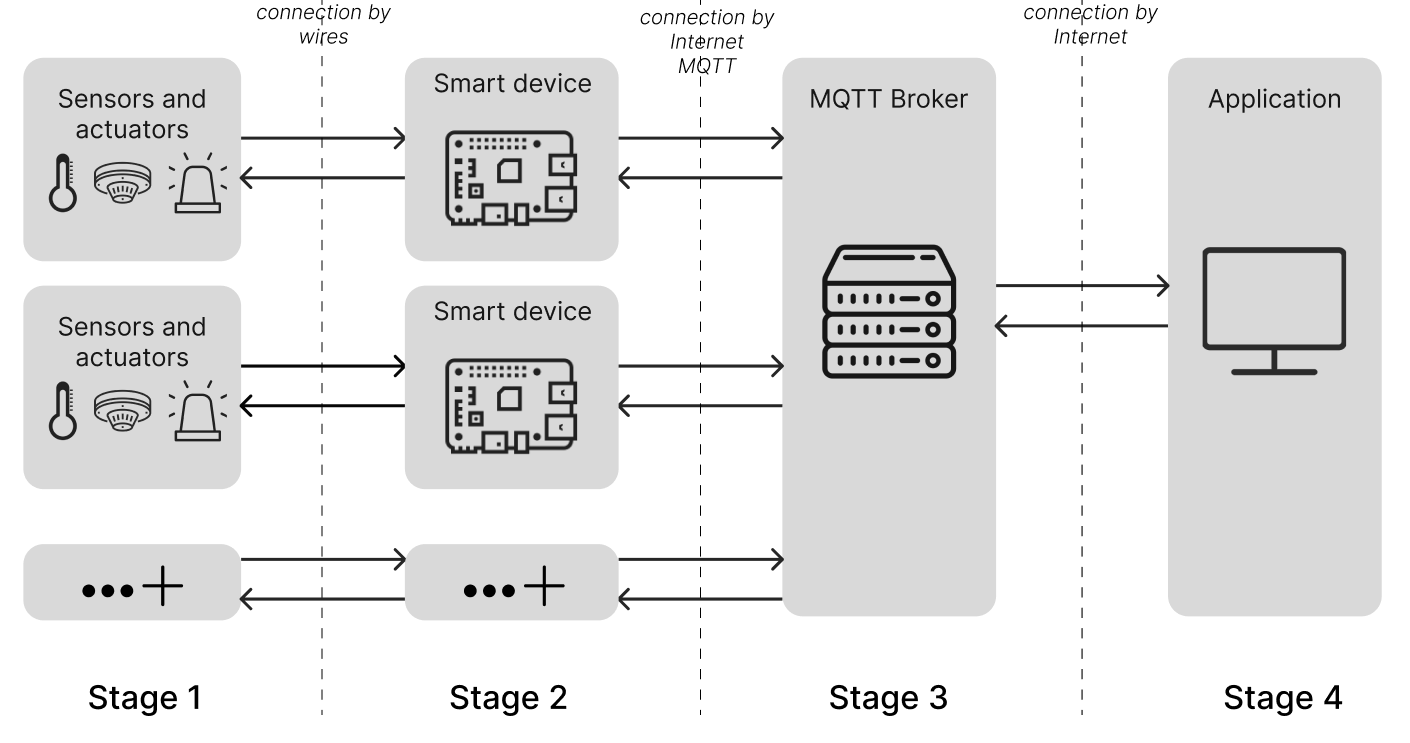
\includegraphics[width=.9\textwidth]{figures/proekt}
    \caption{Koncepcia architektonického modelu projektu \label{proekt}}
\end{figure}
Na obrázku \ref{proekt} si môžete podrobnejšie pozrieť môj koncept. Myslím si, že takéto pomerne štandardné a jednoduché architektonické riešenie bude pre študentov najvhodnejšie na učenie.

%%---------------------------------------------------------------

\subsection{Výber témy pre projekt}
Po vytvorení konceptu som začal premýšľať o konkrétnej téme projektu, ktorá by zodpovedala schéme na obrázku 2. Po dlhom premýšľaní a konzultácii s učiteľom som prišiel s nápadom vytvoriť systém na riadenie mikroklímy skleníkov. 

Podstatou tohto systému je zber údajov o teplote a vlhkosti v skleníkoch, analýza zozbieraných údajov a v prípade, že teplota alebo vlhkosť je mimo normy, potom sa mikroklíma skleníka riadi pomocou aktuátorov, ktoré uvedú ukazovatele do normálu.

Systém sa skladá z nasledujúcich komponentov:
\begin{itemize}
    \item Inteligentné zariadenie, ktoré je umiestnené v skleníku. Jeho úlohou je zber údajov o mikroklíme pomocou senzorov a ich analýza. Ak sú zozbierané údaje mimo normy, zariadenie aktivuje akčne členy, ktoré vyrovnávajú klímu. Všetky zozbierané údaje zo snímačov sa odosielajú na server.
    \item \gls{mqtt} broker, ktorý prijíma údaje, ich prenáša do webovej aplikácie.
    \item Webová aplikácia, ktorá umožňuje regulovať mikroklímu v každom skleníku a zobrazovať aktuálnu teplotu a vlhkosť.
\end{itemize}
Na prvý pohľad je táto myšlienka dobrá a dobre zapadá do koncepcie architektonického modelu (obr. \ref{proekt}), ale zdá sa to tak len na prvý pohľad. Problémy sa začínajú vo fáze rozšírenia implementácie projektu v školách. Teoreticky tento projekt obsahuje nielen senzory, ale aj akčné členy na zmenu teploty a vlhkosti. 

So senzormi by nemali byť žiadne problémy, potrebujeme len senzory svetla a vlhkosti (\gls{ldr} a \gls{dht}) a tie sú už dostupné v štandardných súpravách \textit{Arduino Kit}. Ale s akčnimy členamy je to úplne iná záležitosť. Pri analýze existujúcich riešení podobných nášmu projektu\cite{sklenik1} \cite{sklenik2} \cite{sklenik3}som si uvedomil, že na realizáciu tohto projektu by som potreboval nasledujúce pohony:
\begin{enumerate}
    \item Elektrický motorček (minimálne 12V) na zdvíhanie a spúšťanie okienka.
    \item Počítačový ventilátor na vetranie skleníka.
    \item Elektrické vodné čerpadlo na zvlhčovanie pôdy skleníka.
\end{enumerate}
Tieto komponenty už nie sú súčasťou súpravy \textit{Arduino Kit}, takže školy si budú musieť tieto nástroje zakúpiť dodatočne, čo pre nás nie je veľmi výhodné. Koniec koncov, jednou zo zásad, ktoré chcem pri tvorbe projektu dodržiavať, je minimalizovať dodatočné finančné náklady na kurz. 

Ďalším problémom pri vývoji tohto systému je náročnosť jeho implementácie v školách. Predstavme si, že 20 študentov absolvuje kurz a implementovalo systém podľa návodu. A teraz, aby ste tento systém otestovali, musíte sa veľmi snažiť, pretože školy zvyčajne nemajú niekoľko skleníkov. Samozrejme, môžete sa pokúsiť otestovať systém v rámci jednej alebo viacerých tried, ale podľa môjho názoru je to dosť náročná úloha. 

Vzhľadom na všetky uvedené nevýhody som si uvedomil, že myšlienka vyvinúť systém riadenia klímy v skleníku \gls{iot} nie je relevantná. Myslel som si však, že základ koncepcie je celkom zaujímavý, a tak som na základe predchádzajúcej myšlienky vytvoril novú, ktorá vyriešila všetky predchádzajúce problémy. 

Po niekoľkých ďalších konzultáciách a premýšľaní o možných riešeniach som prišiel s vhodnou myšlienkou bez zjavných nevýhod. Podstatou nového konceptu je vyvinúť systém zberu dát o počasí.

Systém pozostáva z niekoľkých meteorologických staníc navrhnutých študentmi, servera, ktorý zbiera údaje z týchto meteorologických staníc, a webovej aplikácie, z ktorej si môžete pozrieť všetky zozbierané údaje v grafoch, tabuľkách atď. Meteorologická stanica meria teplotu, vlhkosť a svetlo.

Ako vidíte, tento systém je zjednodušenou verziou predchádzajúceho systému. Ako som už napísal vyššie, od predchádzajúcej myšlienky som sa nevzdialil a jednoducho som odstránil komponenty, ktoré s ňou kolidovali, podľa logiky žiadne komponenty, žiadne problémy. Pri analýze predchádzajúceho riešenia som si uvedomil, že hlavným problémom boli pohony, pretože tie projekt úmerne komplikovali. Preto nové riešenie už nemá žiadne pohony, má len najjednoduchšie snímače, ktoré nie je potrebné dokupovať do škôl. 

Napriek tomu, že nové riešenie je trochu zjednodušené, nemyslím si, že by to mohlo nejako ovplyvniť kvalitu vedomostí poskytovaných žiakom. Práve naopak, zjednodušenie hardvéru projektu nám umožní venovať viac pozornosti programovaniu a spracovaniu zozbieraných údajov. Podľa môjho názoru práve toto bude pre mladých programátorov v oblasti internetu vecí užitočnejšie. 
Kvôli prehľadnosti na záver zhrňme tému projektu.

Téma projektu:  Systém na zber údajov o počasí.
Architektúra projektu podľa mojej koncepcie (obr. \ref{proekt}):
\begin{itemize}
    \item Prvá fáza: Senzory tepla, vlhkosti a svetla (\gls{dht}/22, \gls{ldr})
    \item Druhá fáza: Inteligentné zariadenie (ESP32/Raspberry pi)
    \item Tretia fáza: Server, ktorý slúži ako \gls{mqtt} broker
    \item Štvrtá fáza: Webová aplikácia, ktorá zobrazuje všetky zozbierané údaje.
\end{itemize}
Chcem poznamenať, že toto je len teoretický koncept, konečný výsledok sa môže počas vývoja dopĺňať a meniť.

%%---------------------------------------------------------------

\subsection{Výber softvéru a hardvéru na školenie}
Pri čítaní predchádzajúcej časti ste si možno všimli, že použitie takých dosiek ako \textit{ESP32} alebo \textit{Pasbery Py 3/Pico} v projekte môže byť nevhodné a lepším riešením by bolo nahradiť ich \textit{Arduino Uno}. Koniec koncov, \textit{Arduino Uno} je už v školách dostupné, takže nemusíte kupovať nič iné a nebudete musieť študentom vysvetľovať základy používania tohto zariadenia, pretože s ním už pracovali.

A ak vezmeme do úvahy len vyššie uvedené faktory, \textit{Arduino} vyzerá naozaj výhodnejšie v porovnaní s mikrokontrolérmi ako \textit{ESP32} alebo \textit{Raspberry Pi 3/Pico}. Aby som bol úprimný, na začiatku tejto práce som bol tiež fanúšikom používania \textit{Arduina}. V tejto časti však dokážem, prečo bude výber dosky \textit{ESP32} albo \textit{Pasbery Py 3/Pico} v tejto práci vhodnejší, ako rodina dosiek \textit{Arduino}.

Prvá vec, ktorú je potrebné si uvedomiť, je, že vo väčšine štandardných mikrokontrolérov (napr. \textit{ESP32}, \textit{Raspberry Pi 4}, \textit{Raspberry Pi Pico}) už má zabudovaný WiFi modul, zatiaľ čo bežné \textit{Arduina} ho nemajú a preto ich bude treba kúpiť samostatne. Na internete som našiel len niekoľko modelov \textit{Arduina} s integrovaným WiFi modulom, ako napríklad \textit{ARDUINO UNO WiFi REV2}\footnote{\textit{https://store.arduino.cc/products/arduino-uno-wifi-rev2}} a \textit{Arduino Nano RP2040}\footnote{\textit{https://store.arduino.cc/products/arduino-nano-rp2040-connect}}. Avšak v súčasnosti sú tieto zariadenia buď rovnako drahé ako napríklad \textit{ESP32}, alebo niekedy aj drahšie.

Ďalším faktom v prospech doskam tipu \textit{ESP32} je základný programovací jazyk. V prípade rodiny \textit{Arduino} ide zvyčajne o jazyk \textit{C++}, zatiaľ čo u mikroprocesorov je to \textit{Micropython} (takže ten istý \textit{Python}, len s menšou funkcionalitou). Podľa mňa je to dosť dôležitý parameter pre ľahkosť vývoja. Každý, kto už niekedy programoval v jazyku \textit{Micropython}, môže potvrdiť, že programovanie v porovnani s \textit{C++} je oveľa jednoduchšie. Väčšina stredoškolákov už dobre ovláda \textit{Python}, takže programovanie v \textit{Micropythone} by nemalo byť komplikované. Bohužiaľ, v súčasnosti nie sú všetky dosky rodiny \textit{Arduino} podporované \textit{Micropythonom}\footnote{\textit{https://docs.arduino.cc/learn/programming/arduino-and-python}}, existujú len niektoré samostatné platformy, ktoré to môžu. Tieto zariadenia môžete vidieť na obrázku \ref{arduino}. Ako vidíte, v tomto zozname nie je najrozšírenejší Arduino Uno.
\begin{figure}[!ht]
    \centering
    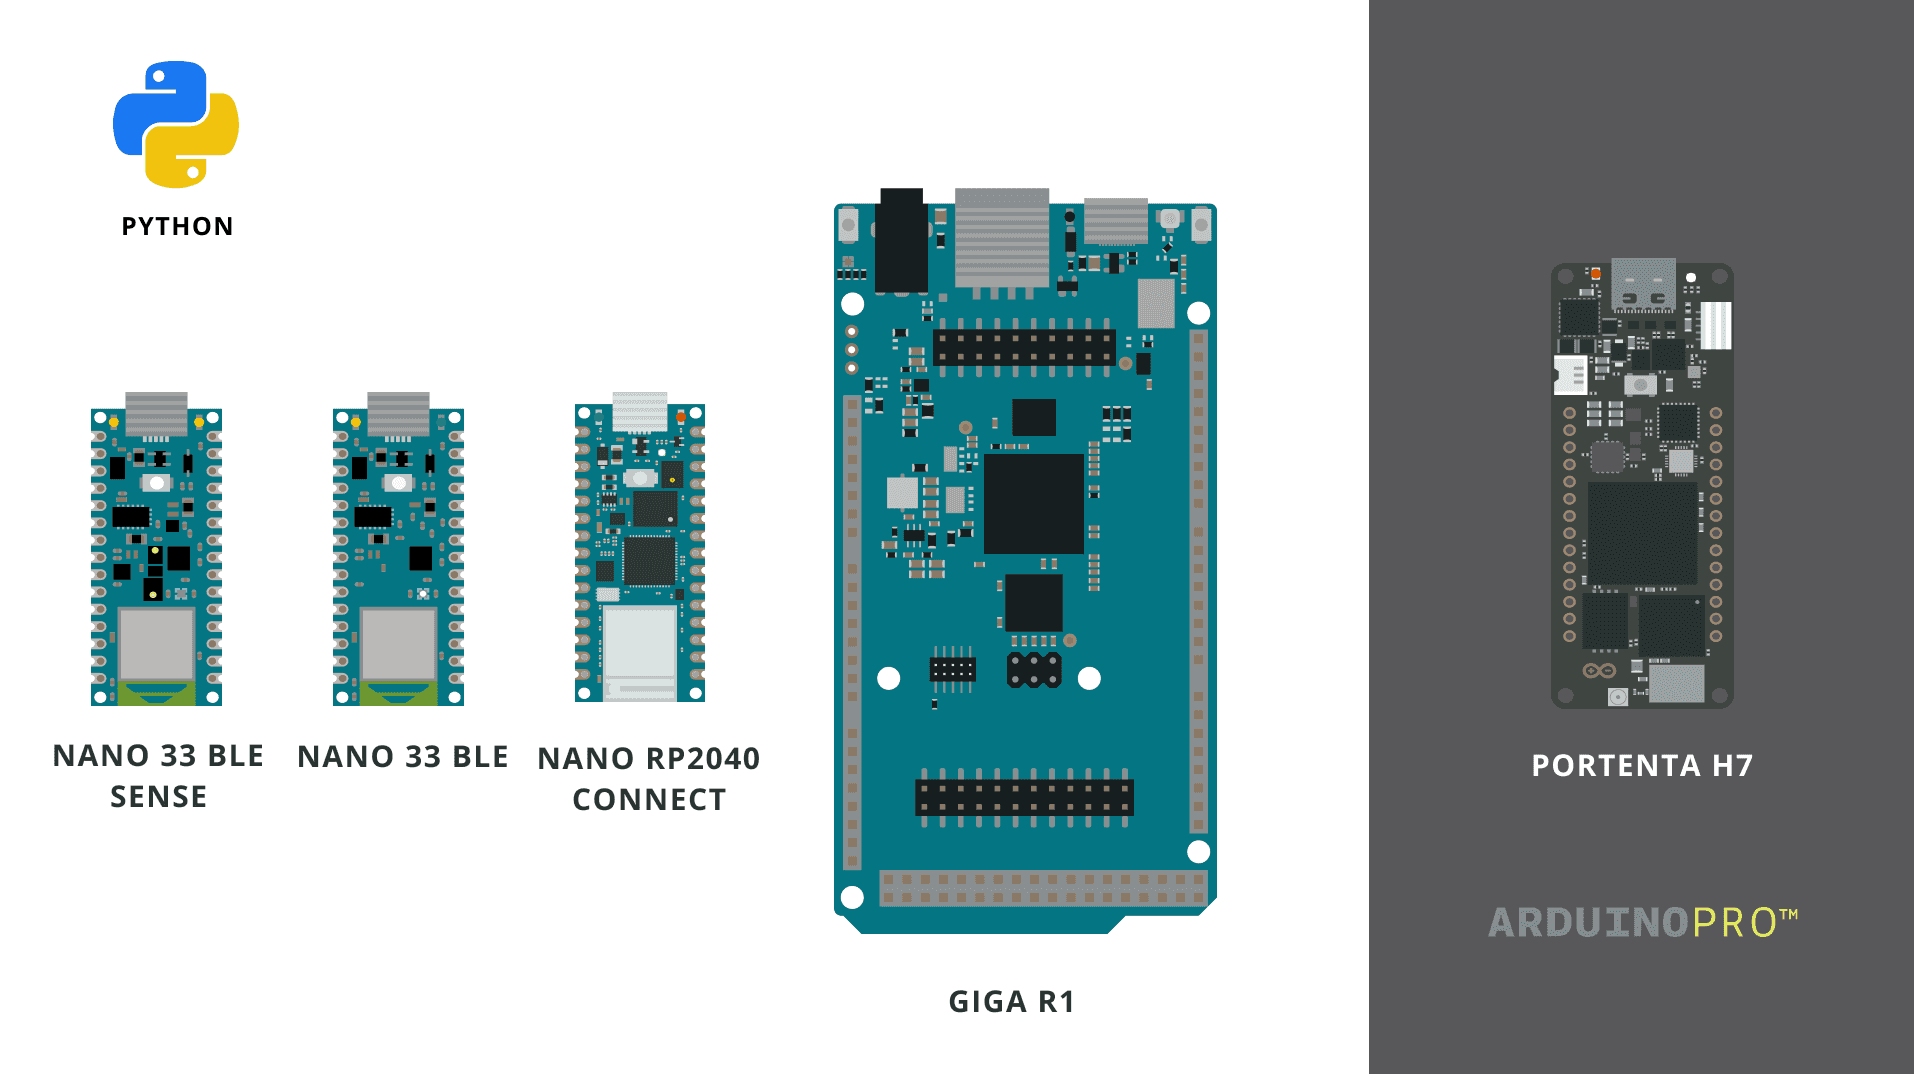
\includegraphics[width=.9\textwidth]{figures/arduino.png}
    \caption{Zoznam platforiem skupiny Arduino, ktoré podporujú Micropython \label{arduino}\cite{arduinoPyt}}
\end{figure}

Chcel by som ešte dodať, že dosky tipu \textit{ESP32} môžu vykonávať širší rozsah úloh než mikrokontroléry, preto výber mikroprocesora ako hlavného zariadenia pre programovanie umožní vyniesť zručnosti študentov na novú úroveň a v budúcnosti budú schopní vykonávať zložitejšie úlohy.


%%---------------------------------------------------------------

\subsection{Výber modelu mikrokontroléra}
Vzhľadom na špecifiká projektových podmienok som hodnotil model mikrokontroléra podľa nasledujúcich kritérií:
\begin{itemize}
    \item Jednoduchosť použitia
    \item Nízka cena
    \item Dostupnosť
\end{itemize}
Ďalším dôležitým parametrom, ktorý by mal byť jednoznačne zahrnutý v doske, je zabudovaný Wi-Fi modul. Zariadenia bez tohto parametru nebudú zvažované. Neberiem do úvahy samostatné čipy, ktoré nie sú pripojené k doske, pretože nie sú absolútne praktické pre prácu s žiakmi stredných škôl.

Ďalej podrobnejšie zanalyzujem jednotlivé kritériá a vyberiem najlepší motel dosky s mikroprocesorom. Začneme s dostupnosťou. Dostupným mikroprocesorom považujem ten, ktorý je ľahko dostupný na globálnom trhu. To znamená model, ktorý nie je deficitný alebo vzácny a je možné ho bez prekážok kúpiť na populárnych internetových obchodoch, ako sú \textit{alza.sk} alebo \textit{aliexpress.com}. Podľa tohto parametra môžem vyzdvihnúť nasledujúce dosky: \textit{ESP32}, \textit{Raspberry Pi 3/4}, \textit{Raspberry Pi Pico W}, \textit{ESP8266}. Na základe svojich skúseností môžem povedať, že najdostupnejšou a najpopulárnejšou voľbou je \textit{ESP32}.

Nasledujúcim kritériom je jednoduchosť použitia. Považujem za logické, ak dáme študentam zariadenie, ktoré bude najviac podobné tomu, čo už poznajú (v tomto prípade \textit{Arduino Uno}). Najvýhodnejšie na tomto poli vyzerá \textit{Raspberry Pi Pico W}, pretože z môjej skúsenosti môžem povedať, že toto zariadenie má najjednoduchšiu prvotnú konfiguráciu zo všetkých modelov, ktoré poznám. Okrem toho, komunikácia s týmto zariadením prebieha cez sériový port, rovnako ako u \textit{Arduino Uno}. Podobné charakteristiky v tejto oblasti má aj \textit{ESP32}, ale treba si uvedomiť, že pre tejto model existuje veľa rôznych konfigurácií, a môj projekt potrebuje štandardizované dosky

Nakoniec sme sa pozreli na otázku ceny. V súčasnosti najlacnejšími modelmi, ktoré som skúmal vyššie, sú \textit{ESP32} (10,81 €)\footnote{\textit{https://rpishop.cz/esp32-a-esp8266/3884-dfrobot-firebeetle-2-esp32-e-iot-mikrokontroler-s-podporou-wi-fi-bluetooth.html}}, \textit{ESP8266} (7,59 €)\footnote{\textit{https://rpishop.cz/esp32-a-esp8266/1944-nodemcu-esp8266-wifi-vyvojova-deska.html}}, \textit{Raspberry Pi Pico W} (7,59 €)\footnote{\textit{https://rpishop.cz/raspberry-pi-pico/5073-raspberry-pi-pico-w-5056561803173.html}}. Všetky ceny som bral z online obchodu \textit{"rpishop.cz"}\footnote{\textit{https://rpishop.cz/}}, pretože tam sú, podľa môjho subjektívneho názoru, dostatočne primerané ceny.

Po zhodnotení všetkých týchto parametrov som dospel k záveru, že Raspberry \textit{Pi Pico W} je najoptimálnejšou voľbou pre túto prácu.

%%---------------------------------------------------------------

\subsection{Dodatočné periférie pre Raspberry Pi Pico W}
Počas jednej z konzultácií mi bolo odporučane pre potreby prace použiť sa na pomocný prvok pre \textit{Raspberry Pi Pico W} s názvom \textit{Cytron Maker Pi Pico Base}\footnote{\textit{https://rpishop.cz/pico-karty/3854-cytron-maker-pi-pico-base-deska-pro-pi-pico-pro-zacatecniky-38515758.html}} (obr. \ref{piPlata}). Ide o pomocnú dosku, ktorej účelom je zjednodušiť pripojenie externých modulov. Skúšal som túto dosku pri vývoji meteorologickej stanice a môžem potvrdiť, že táto pomocná doska skutočne šetrí čas a nervy.

Hlavnou nevýhodou však je, že táto doska je dosť draha, konkrétne 11,02 € za kus. Okrem toho je potrebné dokúpiť špeciálne káble pre pripojenie modulov. Napriek zvýšeniu nákladov projektu, čo je v rozpore s mojím princípom ekonomického prístupu, implementujem túto dosku do kurzu, ale pridám aj možnosť nepoužívať ju na zlacnenie konečného výsledku.

\begin{figure}[!ht]
    \centering
    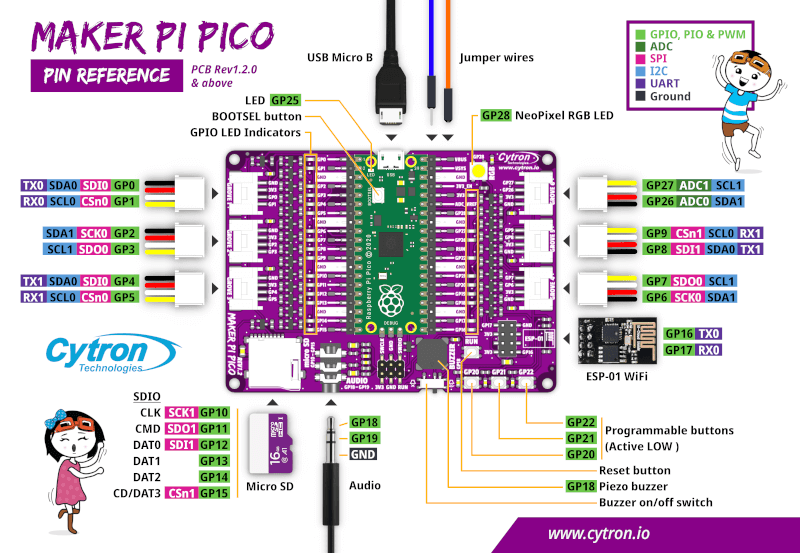
\includegraphics[width=.9\textwidth]{figures/piPlata.png}
    \caption{Vihlad \textit{Cytron Maker Pi Pico Base} \label{piPlata}\cite{cytron}}
\end{figure}

\subsection{Výber \gls{mqtt} brokera}
Zo svojich skúseností s vývojom riešení \gls{iot} môžem povedať, že technológie Hivemq\footnote{\textit{https://www.hivemq.com/}} a Mosquito\footnote{\textit{https://mosquitto.org/}} sú medzi vývojármi najobľúbenejšie. Preto pokladám za logické používať tieto \gls{mqtt} broukery. Ak tieto dve služby zoberieme do úvahy z hľadiska vývoja nášho produktu \gls{iot}, nie je medzi nimi veľký rozdiel. Existuje len malá výhoda Hivemq v podobe príťažlivejšieho webového rozhrania. 

Pri príprave tejto kapitoly som sa zoznámil s študentom Šimonom Pavlišinom, ktorého bakalársky projekt sa týkal vývoja \gls{iot} Gateweja a služby \gls{mqtt} brokera. 

Jeho projekt sa volá \textit{Otvorený \gls{iot} Lab pre stredné školy}\cite{bookSimon} a vyvíja v ňom \textit{Gateway}(ďalej GW) založenú na technológii Mosquito. 

Tento projekt má niekoľko zaujímavých vlastností:
\begin{itemize}
    \item Samotná aplikácia brokera je nainštalovaná na \textit{Raspberry Pi} tretej alebo štvrtej verzie a beží autonómne. Čiže pre lepšie pochopenie si tento projekt môžete predstaviť ako wifi router, ktorý funguje v rámci jedného laboratória alebo učebne, ale namiesto distribúcie wifi slúži ako \gls{mqtt} broker.
    \item Ďalšou vlastnosťou je, že na tomto GW možno vytvárať rôzne aplikácie, ktoré budú bežať paralelne. To sa dosiahne pomocou Doker\footnote{\textit{https://www.docker.com/}} kontajnerov. 
\end{itemize}
Po oboznámení sa s koncepciou projektu Šimona Pavlišina a otestovaní jeho raného prototypu som si uvedomil, že je to presne to, čo potrebujem pre svoju prácu. 

Pre väčšiu istotu uvediem nasledujúce argumenty:
\begin{enumerate}
    \item Možnosť paralelného behu mnohých aplikácií na jednom GW je veľmi silným argumentom pri školení mnohých ľudí.
    \item Už pri práci s raným prototypom tohto projektu som bol presvedčený o jeho použiteľnosti.
    \item Keďže tento GW podporuje Docker, môžem na programovanie aplikácie svojho projektu použiť nastroj NodeRed. Výhody tohto nastroja oproti iným možnostiam opíšem v nasledujúcej časti.
\end{enumerate}
\subsection{Prečo NodeRed?}
Na základe mojich skúseností môžem povedať, že programovanie pmomcou nastroja NodeRed je jedno z najjednoduchších vo svojej oblasti. 

Myslím si, že pri vývoji aplikácie, ktorá je na štvrtej úrovni, je potrebné, aby táto fáza bola čo najjednoduchšia a najľahšia. Podľa môjho názoru je to totiž jedna z najťažších fáz vývoja a myslím si, že ak túto časť príliš skomplikujete, bude materiálu na 5 prednášok príliš veľa. Preto si myslím, že NodeRed bude najjednoduchší a najnázornejší spôsob, ako to urobiť.

% !TEX root = ../thesis.tex
\chapter{Syntetická časť}
\label{methodology}

V tejto časti chcem nielen opísať konečný produkt, ktorý som vytvoril, ale aj celú cestu jeho vývoja. Týmto spôsobom pomôžem čitateľom tejto práce, aby sa pri vývoji podobných vzdelávacích projektov nedopustili podobných chýb.
Vývoj celého projektu som rozdelil do nasledujúcich etáp: 
\begin{enumerate}
    \item Vývoj meteorologickej stanice (1-2 vrstvy architektúry).
    \item Vývoj aplikácie (4. vrstva architektúry).
\end{enumerate}
Samostatnou etapou je testovanie celeho riešenia, ale to bude trochu neskôr.
\section{Počiatočný vývoj meteostanice}
Svoj vývoj som začal od prvých vrstiev podľa konceptu architektúry tohto projektu \ref{iot}, pretože je to pre mňa najlogickejšie riešenie. Preto som ako prvú vec začal vyvíjať meteorologickú stanicu.
\subsection{Prvé pokusy}
Keď som začal pripravovať projekt, nemal som jasný plán postupu ani predstavu o tom, ako by mala meteorologická stanica vyzerať vo svojej konečnej podobe. Kvôli nedostatku skúseností a praktických zručností som mal pri vypracovávaní projektu problémy. Prvé pokusy vývoja boli skôr experimentmi a oboznamovaním sa s výrobným procesom než serióznym vývojom. Po niekoľkých týždňoch takejto neefektívnej práce som však presne pochopil, ako tento projekt vyvíjať a aké základné funkcie musí tento projekt obsahovať. 

Veľmi dôležitú úlohu zohrala skutočnosť, že som pomerne intenzívne komunikoval so svojim veducim praci, ktorý mi v rámci možností radil vo všetkých otázkach, ktoré ma v súvislosti s procesom vivoja zaujímali.

Na začiatku vývoja projektu som používal \textit{Raspberry Pi Pico WH} a všetky pripojenia modulov som robil na \textit{breadboarde} (obr. \ref{breadboard}). Ale po čase som na uľahčenie vývoja začal používať \textit{Cytron Maker Pi Pico Base}.

\begin{figure}[!ht]
    \centering
    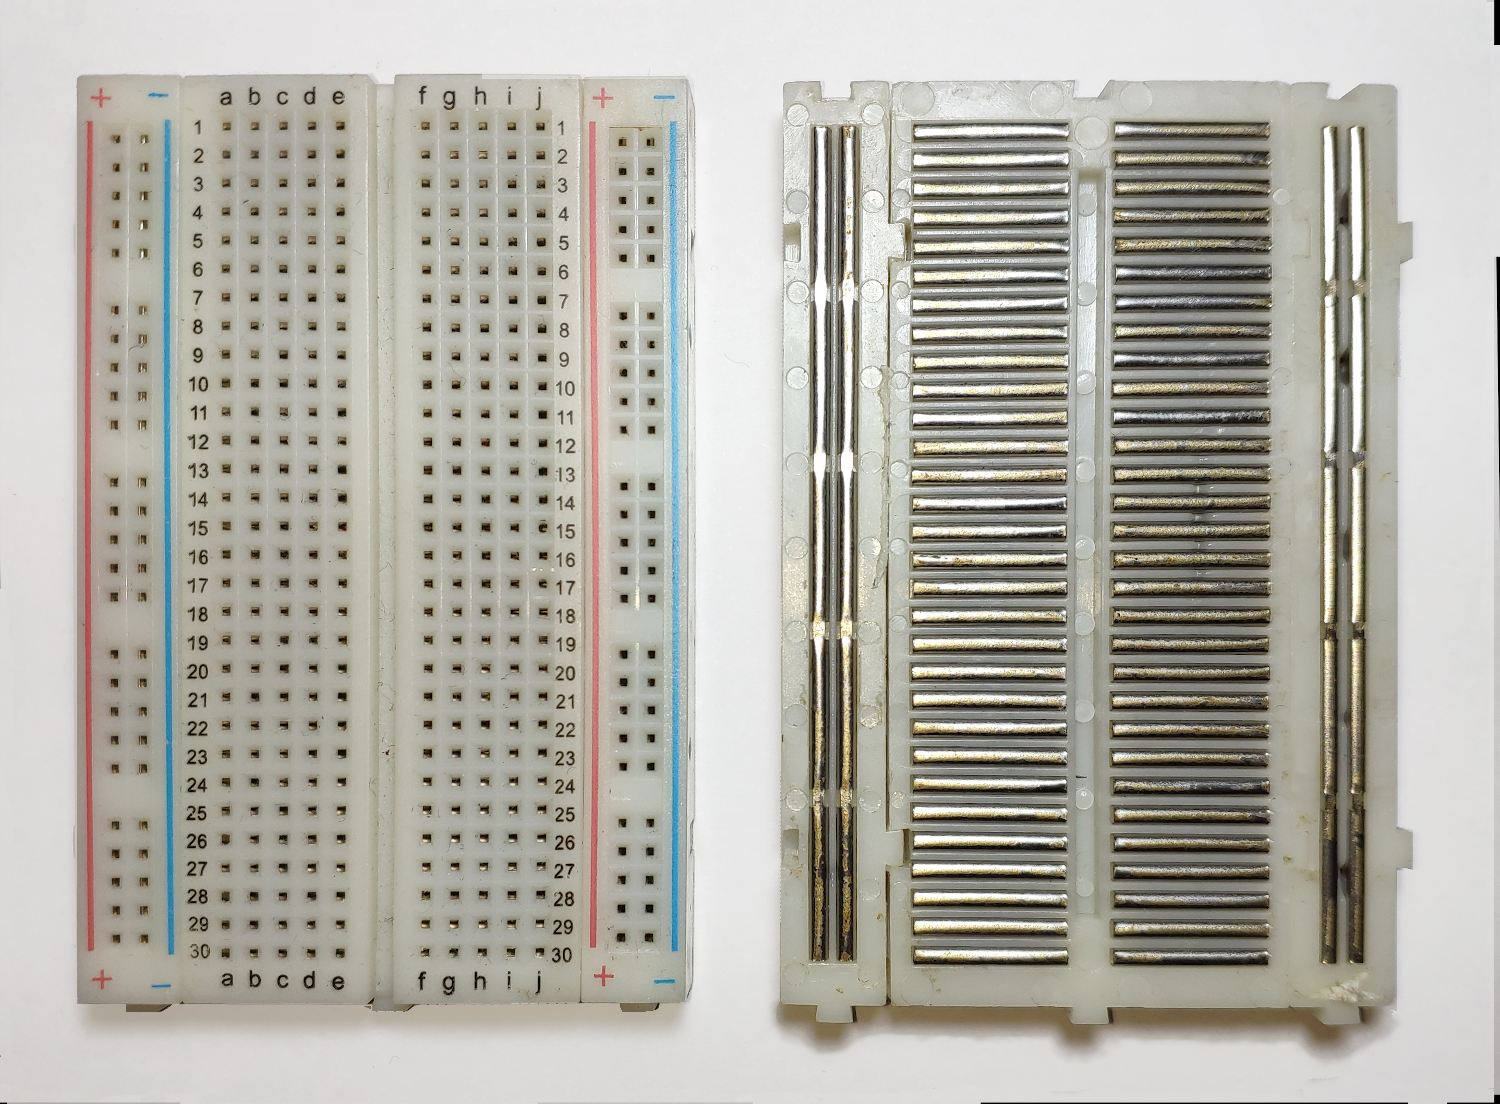
\includegraphics[width=\textwidth]{figures/breadboard}
    \caption{Vzhľad breadboardu z oboch strán\label{breadboard}\cite{breadboard}}
\end{figure}

\subsection{Zásady vývoja}
Pre správne splnenie úloh, musel som si vytvoriť podrobný, postupný plán činnosti pre vývoj meteostanice. 

Po premyslení tohto problému som prišiel s nasledujúcim akčným plánom:
\begin{enumerate}
    \item Vytvoriť hardvérovú časť meteostanice, konkrétne:
    \begin{itemize}
        \item Model toho, čo by mala táto meteorologická stanica obsahovať.
        \item Nakresliť elektricky obvod na pripojenie modulov.
        \item Vykonanie schémy na reálnom príklade.
    \end{itemize}
    \item Vytvoriť softvérovú časť meteorologickej stanice a implementovať nasledujúce funkcie:
    \begin{itemize}
        \item Zber údajov zo senzorov.
        \item Odosielanie údajov na \gls{mqtt} broker.
        \item Úspora energie (zabezpečiť možnosť autonómie).
        \item Tolerancia porúch.
        \item Dodatočné fičury.
    \end{itemize}
\end{enumerate}

%%------------------------------------------------------------------------

\section{Hardvérová časť meteostanice}
Meteorologická stanica by mala odčítať nasledujúce údaje: 
\begin{itemize}
    \item Teplota
    \item Vlhkosť vzduchu
    \item Intenzita svetla
\end{itemize}
Na tieto úlohy som použil senzor \gls{ldr} (intenzita svetla) a \gls{dht} (teplota a vlhkosť). Namiesto \gls{dht} by bolo možné použiť samostatné snímače teploty a vlhkosti, ale to je zbytočná komplikácia procesu vývoja. Namiesto \gls{dht} je môžne použiť novšiu verziu DHT22. V ich zapojení nie je osobitný rozdiel, ale na softvérovej úrovni novšia verzia používa inú knižnicu.

Počas priameho vývoja som sa stretol s problémom, že počas autonómnej prevádzky zariadenia nie je jasné, či funguje alebo má problém. Preto som do zariadenia pridal \gls{led} diódu, ktorá informuje vývojára o stave meteostanice.

Na pripojenie k \textit{Raspberry Pi Pico} budete potrebovať dva rezistory,
a to 10k$\Omega$
  a 220k$\Omega$.

  Konečný zoznam použitých komponentov je tu:
\begin{itemize}
    \item \gls{dht} 
    \item \gls{ldr}
    \item \gls{led} dióda
    \item 10k$\Omega$ rezistor
    \item 220k$
    \Omega$ rezistor
\end{itemize}
Na obrázku \label{schema} vidíme schému pripojenia všetkých modulov k doski \textit{Raspberry Pi Pico}. 

\subsection{Schéma zapojenia}
Ako už bolo opísané v teoretickej časti, projekt bude vyvinutý na základe doski \textit{Raspberry Pi Pico W}. Preto bola všetka práca vykonaná na tejto doske. Ale ja som otestoval fungovanie svojho projektu aj na \textit{ESP32} so zabudovaným WiFi modulom a môžem povedať, že som žiadne problémy nezistil. 

Preto sa v prípade potreby môže projekt realizovať aj pomocov doski na báze čipu \textit{ESP32}, a nie \textit{Raspberry Pi Pico W}. Chcem však upozorniť, že pred vedením kurzu musí učiteľ dôkladne otestovať verziu \textit{ESP32}, ktorú majú študenti k dispozícii, pretože existuje veľa konfigurácií dosiek s čipom \textit{ESP32} a ja nemôžem zabezpečiť fungovanie projektu na každej z nich. To znamená, že \textit{Raspberry Pi Pico W} je zárukou, že všetko bude fungovať tak, ako som ako vývojár zamýšľal. 

Ak sa teda vrátime k téme pripojenia jednotlivých modulov k doske mikroprocesora, potrebujeme dva digitálne piny na pripojenie diódy a \gls{dht} a jeden analógový pin na pripojenie \gls{ldr} senzora. Je potrebné poznamenať, že \gls{ldr} senzory sú dvoch typov, s digitálnymi a analógovými výstupmi. V projekte možno použiť obe verzie, ale je potrebné zohľadniť rozdiel v ich pripojení na softvérovej úrovni. Ja použijem analógovú verziu \gls{ldr}, pretože je súčasťou \textit{Arduino Kit}.

\begin{figure}[!ht]
    \centering
    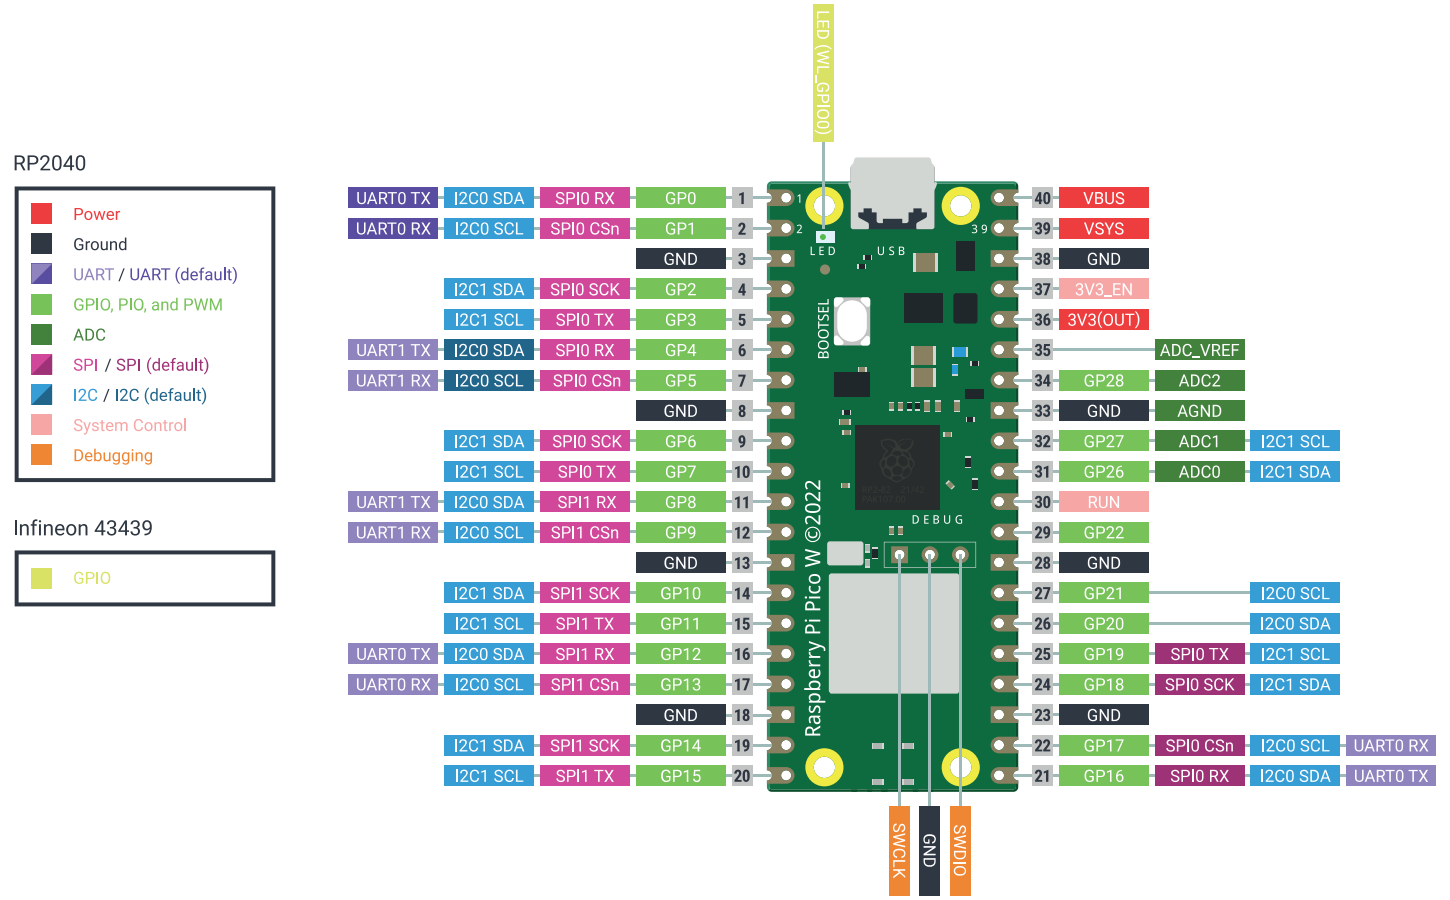
\includegraphics[width=\textwidth]{figures/raspberry_pi_pico}
    \caption{Rozloženie pinov na doske \textit{Raspberry pi pico W} \label{pico} \cite{piPico}}
\end{figure}

Ako vidne na obrázku \ref{pico}, \textit{Raspberry Pi Pico W} má iba tri analógové piny, a to: GP26, GP27, GP28. Môžete použiť ktorýkoľvek z nich, ja použijem GP26. Na pripojenie \gls{dht} a \gls{led} diódy môžete použiť ktorýkoľvek z dostupných digitálnych pinov, ja použijem GP21, a GP20. Na obrázku \ref{schema} môžete vidieť celú schému pripojenia k mikroprocesoru \textit{Raspberry Pi Pico W}. 

\begin{figure}[!ht]
    \centering
    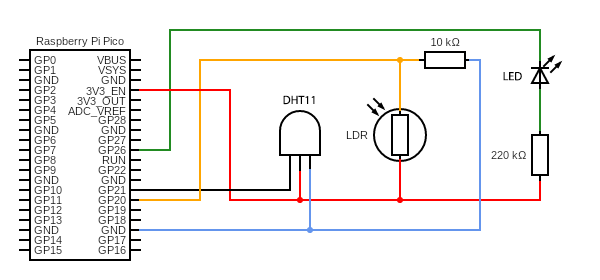
\includegraphics[width=\textwidth]{figures/circuit}
    \caption{Chéma pripojenia k doske Raspberry pi pico W \label{schema}}
\end{figure}

Dodatočne by som chcel upozorniť, že schéma zapojenia znázornená na obrázku \ref{schema} môže byť v niektorých prípadoch nefunkčná, pretože počet pinov na rôznych verziách modulov (napr. \gls{dht}) sa môže líšiť od toho, čo som uviedol. Preto by mal učiteľ pred vedením kurzu skontrolovať existujúcu konfiguráciu modulov a v prípade potreby zmeniť schému zapojenia.

\subsection{Príklady realizácie schémy zapojenia}
Celkovo som tento schému (obrázok\ref{schema}) realizoval v troch formách:
\begin{enumerate}
    \item Pomocou \textit{Raspberry Pi Pico W} (obrázok \ref{f_pico}).
    \item Pomocou \textit{Raspberry Pi Pico W} s použitím \textit{Cytron Maker Pi Pico Base W} (obrázok \ref{f_b_pico}).
    \item Pomocou \textit{ESP32} (obrázok \ref{f_esp32}). 
\end{enumerate}

Ako je môžne vidieť na obrázkoch \ref{f_pico} a \ref{f_esp32}, medzi vzhľadom pripojenia \textit{ESP32} a \textit{Raspberry Pi Pico W} nie je veľký rozdiel. Najjednoduchšie sa pripájal \textit{Raspberry Pi Pico W} s pomocnou doskou (obr. \ref{f_b_pico}), pretože nebolo potrebné použiť dodatočné rezistory ani veľké množstvo káblov.

Môžem tiež poznamenať, že schéma rozpojenia na obrázku \ref{schema} je len príkladom a ak spojenie urobíte trochu inak pri dodržiavaní logiky spojenia, nemali by vzniknúť žiadne problémy.

Pri práci s mikroprocesormi je dôležité dodržiavať bezpečnostné pravidlá, konkrétne zabrániť skratom pri zostavovaní fyzickej kópie projektu. Pri práci s ESP32 som kvôli nedostatku skúseností spálil mikroprocesor skratom. Viac takýchto incidentov som už nepripustil.

\begin{figure}[!ht]
    \centering
    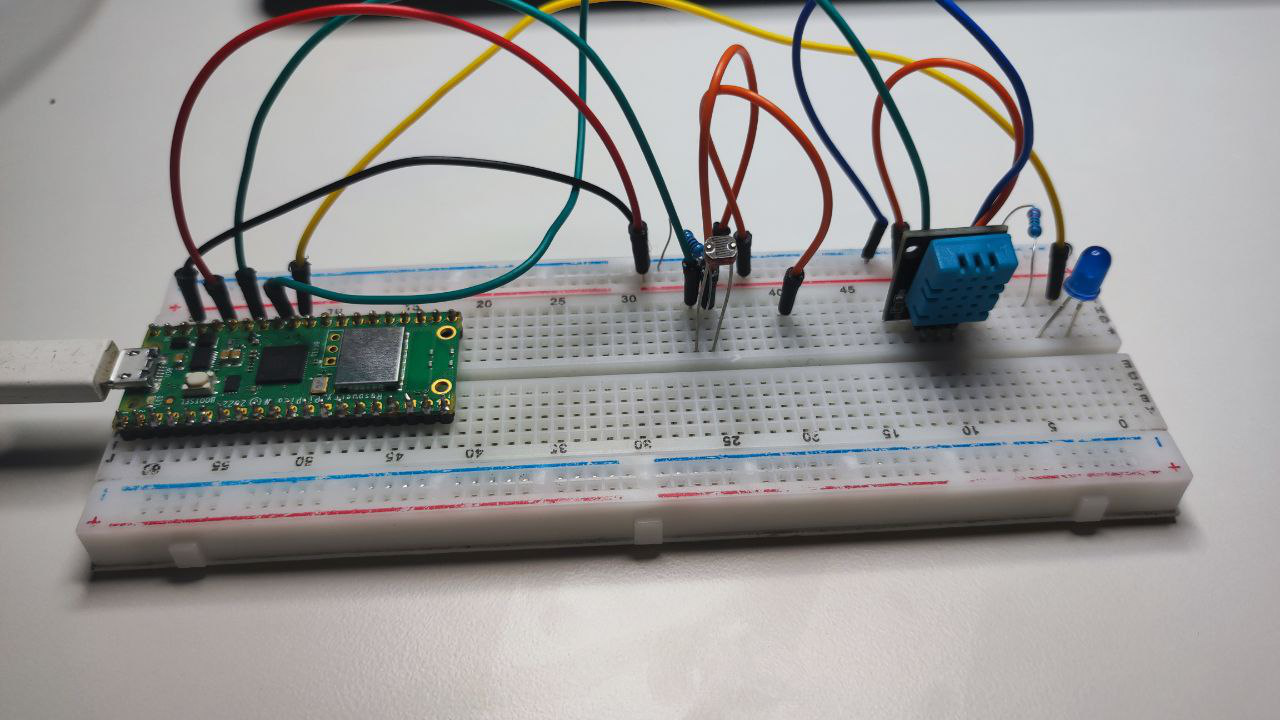
\includegraphics[width=\textwidth]{figures/f_pico}
    \caption{Fyzický príklad schémy zapojenia \ref{schema} pomocou \textit{Raspberry Pi Pico W} \label{f_pico}}
\end{figure}

\begin{figure}[!ht]
    \centering
    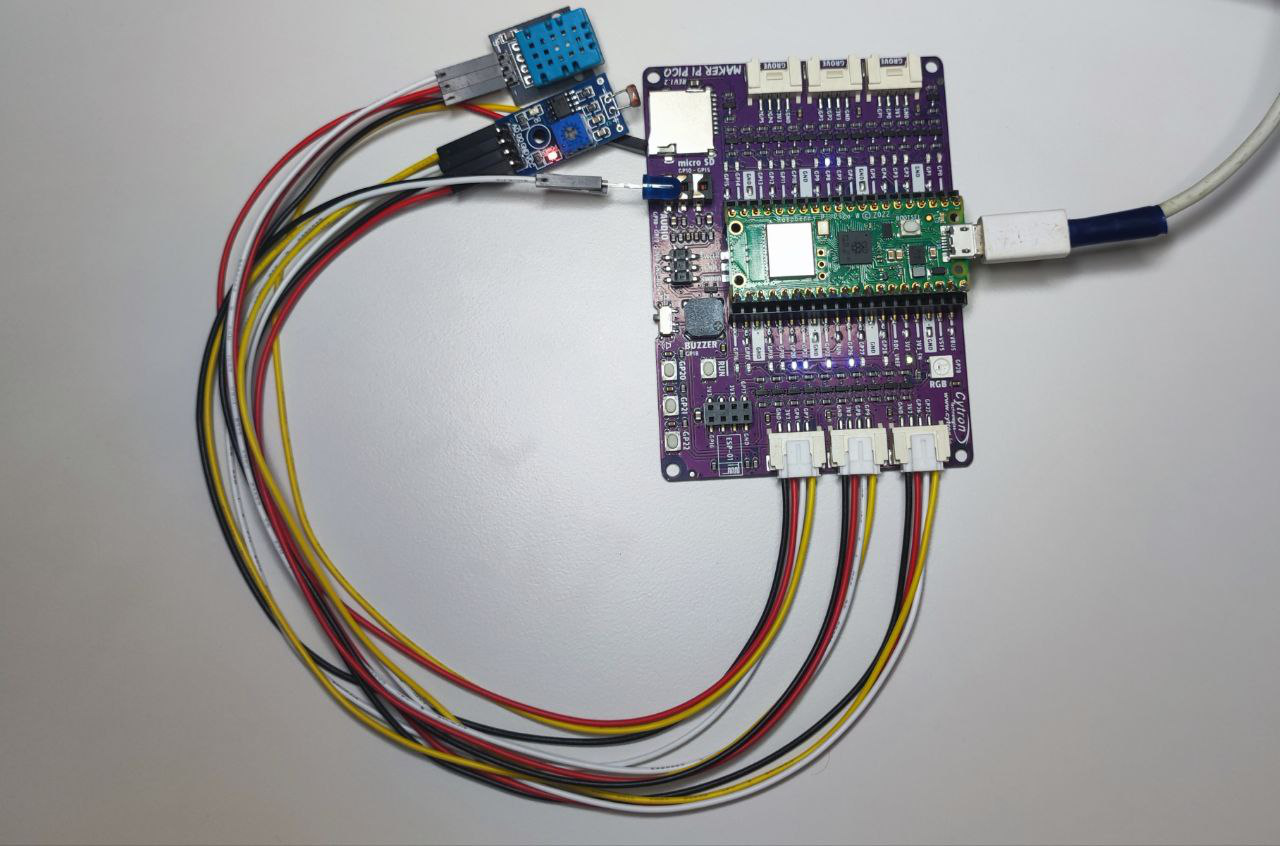
\includegraphics[width=\textwidth]{figures/f_bord_pico}
    \caption{Fyzický príklad schémy zapojenia \ref{schema} pomocou \textit{Raspberry Pi Pico W} s doplnkovou doskou \textit{Cytron Maker Pi Pico Base}\label{f_b_pico}}
\end{figure}

\begin{figure}[!ht]
    \centering
    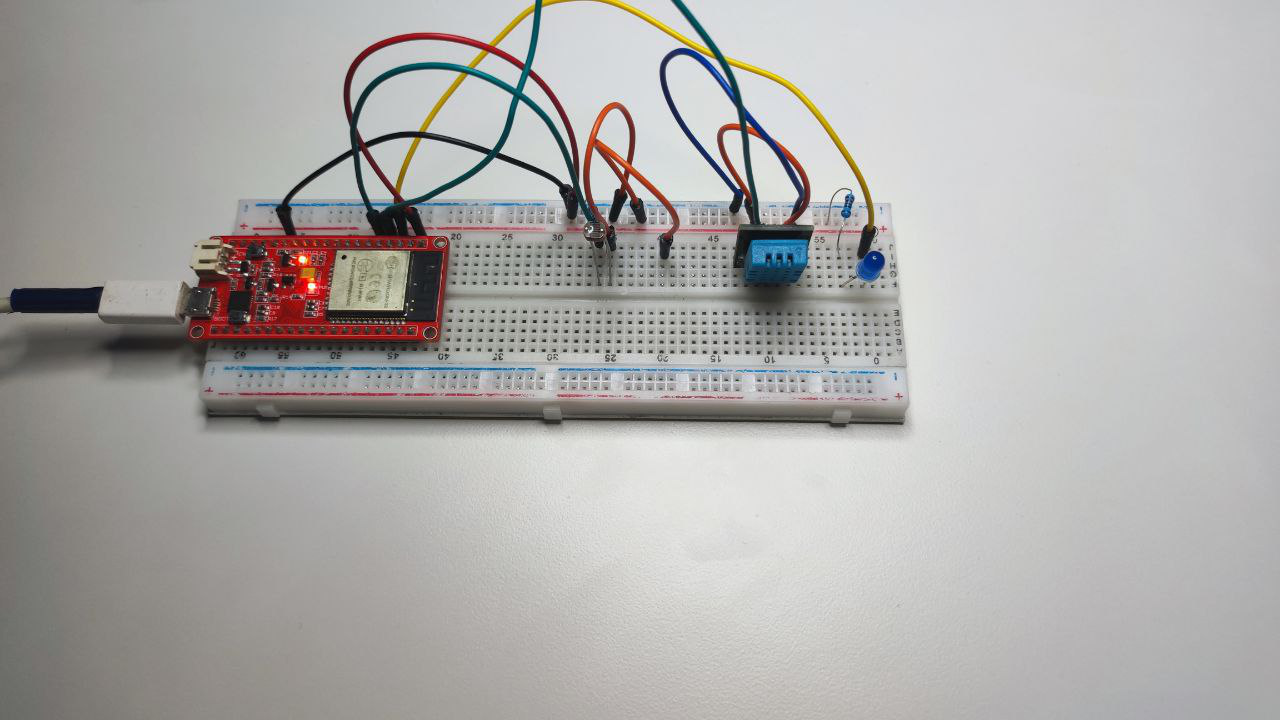
\includegraphics[width=\textwidth]{figures/f_esp32}
    \caption{Fyzický príklad schémy zapojenia \ref{schema} pomocou \textit{ESP32} \label{f_esp32}}
\end{figure}

%%------------------------------------------------------------------------

\section{Vývoj softvérovej časti meteostanice}
Softvér bol napísaný v programovacom jazyku \textit{MicroPython}, ako bolo napísané v predchádzajúcich častiach bakalárskej práce. 

Softvér pre meteorologickú stanicu bol vyvinutý v troch iteráciách:
\begin{enumerate}
    \item Počiatočné vytvorenie kódu so všetkými potrebnými funkciami.
    \item Refaktoring.
    \item Testovanie.
\end{enumerate}
V nasledujúcich podkapitolách podrobnejšie opíšem každú z týchto fáz.

\section{Hlavná časť vývoja (Prvá iterácia)}
\subsection{Postup vývoja}
V prvej iterácii vývoja kódu som sa nestaral o čistotu kódu a nerobil som žiadny refaktoring. To mi umožnilo sústrediť sa na samotný vývoj. 

Počas vývoja kódu som postupne pridával nové funkcie do meteorologickej stanice a snažil som sa dodržať vyššie uvedený plán vývoja. 

Pozrime sa na celý vývojový cyklus prvej iterácie a podrobnejšie rozoberme jednotlivé fázy pridávania nových funkcií pri zachovaní časovej hierarchie pridávania do projektu:
\begin{enumerate}
    \item \textit{Čítanie senzorovych dát} - implementoval som možnosť čítať metriky vlhkosti, teploty a svetla zo senzora \gls{ldr} a \gls{dht}. 
    
    Aby som zabránil načítaniu nesprávnych informácií, odčítam údaje 3-krát a vypočítam z nich medián. Ak sa teda z nejakého neznámeho dôvodu jedenkrát odčítajú nesprávne údaje, v nasledujúcich krokoch sa nezohľadnia.
    
    \item \textit{Pripojenie k internetu} - táto fáza bola najjednoduchšia na realizáciu.
    \item \textit{Pripojenie k \gls{mqtt}} - na implementáciu tejto a ďalšej etapy som použil knižnicu tretej strany, pretože základný balík \textit{Micropythonu} neobsahoval knižnicu, ktorú som potreboval. 
    \item \textit{Odoslanie údajov} - zozbierané a spracované údaje z prveho kroku sa odošlú do sprostredkovateľa \gls{mqtt}. 
    
    V počiatočných fázach som údaje posielal vo forme troch čísel, ale časom som si uvedomil, že tento typ údajov sa dosť ťažko číta, preto som začal údaje posielať vo forme \gls{json} správy.
    \item \textit{Šetrenie energie} - keďže meteorologická stanica má byť autonómna, šetrenie energie je dôležitou súčasťou tohto produktu. 
    
    Šetrenie energie som realizoval znížením taktu procesora, alebo takzvaným \textit{uspávaním} mikroprocesora. Dosahuje sa to pomocou špeciálnych príkazov a v prvých fázach vývoja som používal funkciu \verb|sleep()|, ktorá pozastaví aktuálny proces, čím sa zníži zaťaženie procesora. V budúcnosti som ju však nahradil energeticky úspornejšou funkciou \verb|deepsleep()|, ktorá zastaví všetky aktuálne procesy a prejde do úsporného režimu. 
    
    Túto fázu som vyvinul na základe týchto uvedených experimentov\cite{spotrebaEnergie1}\cite{spotrebaEnergie2}\cite{spotrebaEnergie3}.
    \item \textit{Problémová signalizácia} - ak meteorologická stanica nie je pripojená k počítaču, spotrebiteľ alebo vývojár nemá možnosť zistiť aktuálny stav systému bez prístupu k sériovému portu. Preto som sa v tomto bode rozhodol pridať \gls{led} diódu, ktorá bude signalizovať aktuálny stav zariadenia. 
    
    Teraz počas prevádzky zariadenia dióda signalizuje úspešnosť takých akcií, ako napr: 
    \begin{itemize}
        \item Pripojenie k wifi. 
        \item Pripojenie k sprostredkovateľovi \gls{mqtt}.
        \item Odosielanie údajov.
    \end{itemize}
    
    Ak dióda svieti 5 sekúnd, akcia bola úspešná, a ak bliká, akcia sa nepodarila. Na lepšie označenie problémov možno čas blikania a ich počet pre jednotlivé akcie meniť. 
    \item \textit{Tolerancia porúch} - počas prevádzky meteostanice existuje možnosť, že pripojenie k internetu alebo k serveru \gls{mqtt} sa môže z nejakých príčin prerušiť. 
    
    V čase takýchto problémov s pripojením môže dôjsť k strate zozbieraných údajov, pretože sa nebudú môcť dostať na server. Preto som sa rozhodol tento problém vyriešiť nasledujúcim spôsobom. 
    
    Pred odoslaním údajov sprostredkovateľovi \gls{mqtt} program skontroluje sieťové pripojenie a ak nie je dostupné, uloží zozbierané údaje do buffer súboru. Ak sa internetové pripojenie počas nasledujúcich iterácií opäť objaví, všetky údaje, ktoré sa nahromadili v súbore, sa odošlú na server. Toto je pomerne jednoduchý, ale účinný algoritmus.
    \item \textit{Aktualizácia času} - pri vývoji predchádzajúceho kroku som narazil na problém, že odoslané údaje sa nedajú rozlíšiť podľa času ich načítania. To znamená, že strana servera nerozumie presnému času merania a potenciálny spotrebiteľ môže analyzovať údaje len podľa času ich odoslania na server. 
    
    Preto som do \gls{json} správy, ktorá sa posiela na server, pridal parameter \verb|time|, ktorý znamená presný čas tohto merania v UTC.  Narazil som však na ďalší problém. Konkrétne na problém kontextualizácie času. 
    
    Ak je aplikácia spustená cez \gls{ide}(napr. \textit{Thonny}), tak by nemal nastať žiadny problém, pretože \gls{ide} automaticky aktualizuje čas na mikroprocesore, ale ak je aplikácia spustená bez mikroprocesora, tak sa čas neaktualizuje a nastaví sa na začiatok éry\footnote{\textit{https://docs.micropython.org/en/latest/library/time.html}}(1970-01-01 00:00:00 UTC). Preto som do programu implementoval automatickú aktualizáciu času, ale na jej vykonanie je potrebné mať prístup na internet. 
\end{enumerate}
\subsection{Pomocná knižnica}
Pri vývoji softvéru pre meteorologickú stanicu ma napadlo vytvoriť samostatnú knižnicu s funkciami, o ktorých predpokladám, že by mohli byť pre študentov s malými skúsenosťami s programovaním dosť náročné. Mohla by tiež obsahovať niektoré funkcie, ktoré štandardizujú údaje.

Vytvoril som teda takúto knižnicu a pomenoval som ju \verb|helper.py|.

Táto knižnica obsahuje nasledujúce funkcie:
\begin{itemize}
    \item \verb|def do_connect_wifi(ssid, password)| - Pripája sa k zadanej sieti WiFi. \\Vráti: \verb|True|, \verb|False|.(v závislosti od úspešnosti pripojenia)
    \item \verb|def do_connect_broker(name, server, port, login, password)| - Pripája k \gls{mqtt} brokeru. \\Vráti: Objekt \gls{mqtt} brokera, \verb|None|.(v závislosti od úspešnosti pripojenia)
    \item \verb|def send_mqtt_mesage(mqtt, topic, mesage)| - Odošle správu na zadaný \gls{mqtt} broker. \\Vráti:  \verb|True|, \verb|False|.(v závislosti od úspešnosti pripojenia)
    \item \verb|def create_json(time, temperature, humidity, light)| - Konvertuje zadané údaje do formatu \gls{json}. \\Vráti: \gls{json} v textovej forme. \\Tento príkaz slúži na štandardizáciu správ odosielaných na \gls{mqtt} server.
    \item \verb|def read_light(adc_pin)| - Meria osvetlenie z daného pinu. \\Vráti: Percent osvetlenia od 0 do 100. 
\end{itemize}

\subsection{Kritické problémy, s ktorými som sa stretol počas vývoja.}
Ako som už napísal, pri práci s mikroprocesormi je potrebné dodržiavať bezpečnostné opatrenia, aby ste predišli rôznym nepríjemným situáciám. Pri vývoji softvéru sa však vývojár môže dopustiť niektorých nezrejmých chýb, ktoré môžu viesť k úplnej strate kódu, alebo dokonca firmvéru. Počas svojej práce som sa s jedným takýmto problémom stretol a v tejto časti ho opíšem, aby prípadný čitateľ tejto práce neurobil podobnú chybu.

Dovoľte mi teda uviesť stručný prehľad tohto problému. Pri opise vývoja som v časti o šetrení energie písal o vhodnejšom použití funkcie \verb|deepsleep()| namiesto funkcie \verb|sleep()|. Počas aktívneho vývoja, keď má váš kód nejaké problémy, sa však pri použití funkcie \verb|deepsleep()| môže váš kód dostať do tzv. $"$dead loop$"$. Zvyčajne sa problémy s $"$dead loop$"$ riešia reštartovaním systému, ale nie v prípade funkcie \verb|deepsleep()|. Aby fungovala správne, hlavný súbor vašej aplikácie sa musí volať start.py, to znamená, že je to súbor, ktorý sa spustí pri každom zapnutí mikroprocesora. 

Riešením tohto problému je úplné prepísanie systému mikroprocesora. Možno existujú humánnejšie spôsoby riešenia tohto problému, ale v mojom prípade je to jediný spôsob, ktorý som mohol urobiť. 

Aby ste tomuto problému predišli, odporúčam vám používať funkciu deepsleep() až v záverečných fázach, keď ste si istí, že program pracuje správne. V počiatočných fázach vývoja vám odporúčam používať funkciu \verb|sleep()|.

\subsection{Výsledok vývoja a potreba refaktoringu.}
Takže keď som implementoval všetky potrebné funkcie a vyriešil som všetky problémy súvisiace s vývojom meteostanice, získal som produkt, ktorý cyklicky vykonáva tieto kroky:
\begin{itemize}
    \item Prebudí sa a pripojí sa k sieti.
    \item Sníma a odosiela údaje na server. 
    \item Zaspí na 5 minút.
\end{itemize}

Je to veľmi jednoduchý algoritmus, ale pre meteostanicu nepotrebuje nič viac. V tejto etape už teda projekt vyzerá viac-menej dobre, takže je čas premýšľať o tom, ako budú môcť študenti realizovať projekt.

Po zamyslení sa nad touto otázkou som dospel k záveru, že na to, aby študenti mohli pracovať efektívne, je potrebné vytvoriť kostru projektu, na základe ktorej budú študenti vykonávať ďalší vývoj. To znamená, že namiesto toho, aby študenti robili všetko od začiatku, budú mať základ projektu a zoznam funkcií, ktoré musia urobiť. Pri tejto metóde študenti strácajú pocit neurčitosti a nepochopenia, a tak sa kód študentov stáva štandardizovanejším, čo zlepšuje možnosť hodnotenia. 

Koreň projektu je logické vytvoriť na základe už hotového projektu, teda toho, čo som už urobil. Je tu však jeden problém, momentálne je môj kód pre meteorologickú stanicu veľmi hrubý a neprehľadný na čítanie. Preto som dospel k záveru, že softvér, ktorý som vytvoril, je potrebné refaktorovať.

%%------------------------------------------------------------------------

\section{Refaktoring (Druhá iterácia)}
Takže v čase, keď som začal refaktorovanie, vyzeral môj projekt takto: 
\begin{itemize}
    \item \verb|main.py| - tu sa nachádza hlavná časť kódu. 
    \item \verb|helper.py| - pomocná knižnica, o fungovaní ktorej som už písal.
\end{itemize}

Kód v súbore \verb|main.py| bol pred refaktorovaním veľmi neprehľadný a bolo veľmi ťažké identifikovať funkcie, ktoré by mohli byť súčasťou kostry projektu. Preto bolo rozhodnuté rozdeliť kód v tomto súbore na niekoľko častí.

Počas jednej z konzultácií mi učiteľ Miroslav Biňas vnukol myšlienku, že proces fungovania meteostanice možno reprezentovať ako konečný stavový automat a kód projektu možno rozdeliť do jednotlivých stavov projektu. Táto myšlienka sa mi zdala naozaj veľmi chytrá, preto som kód projektu zmapoval na tento model. V nasledujúcich kapitolách budem podrobnejšie hovoriť o tom, ako tento koncept vyzerá a aký bol konečný výsledok.

\subsection{Konečný stavový automat v projekte}
Konečný stavový automat je koncept, ktorý opisuje veci v zmysle jednotlivých stavov a počet týchto stavov je konečný\cite{KA}. V našom prípade použijem tento pojem na opis cyklickej logiky meteostanice v rámci jednotlivých stavov.

Analyzoval som logiku meteostanice a identifikoval som nasledujúce stavy:
\begin{itemize}
    \item Inicializácia - zariadenie sa pripojí k wifi a \gls{mqtt} brokeru.
    \item Meranie - zariadenie meria parametre teploty, vlhkosti a svetla.
    \item Odosielanie - zozbierané údaje sa spracujú a odošlú na server \gls{mqtt}.
    \item Uspanie - zariadenie prejde do energeticky efektívneho režimu na konštantný čas.
\end{itemize}
Všetky tieto stavy sa cyklicky striedajú jeden za druhým donekonečna. Na obrázku \ref{ksa} môžete vidieť, ako vyzerajú vo forme diagramu.
\begin{figure}[!ht]
    \centering
    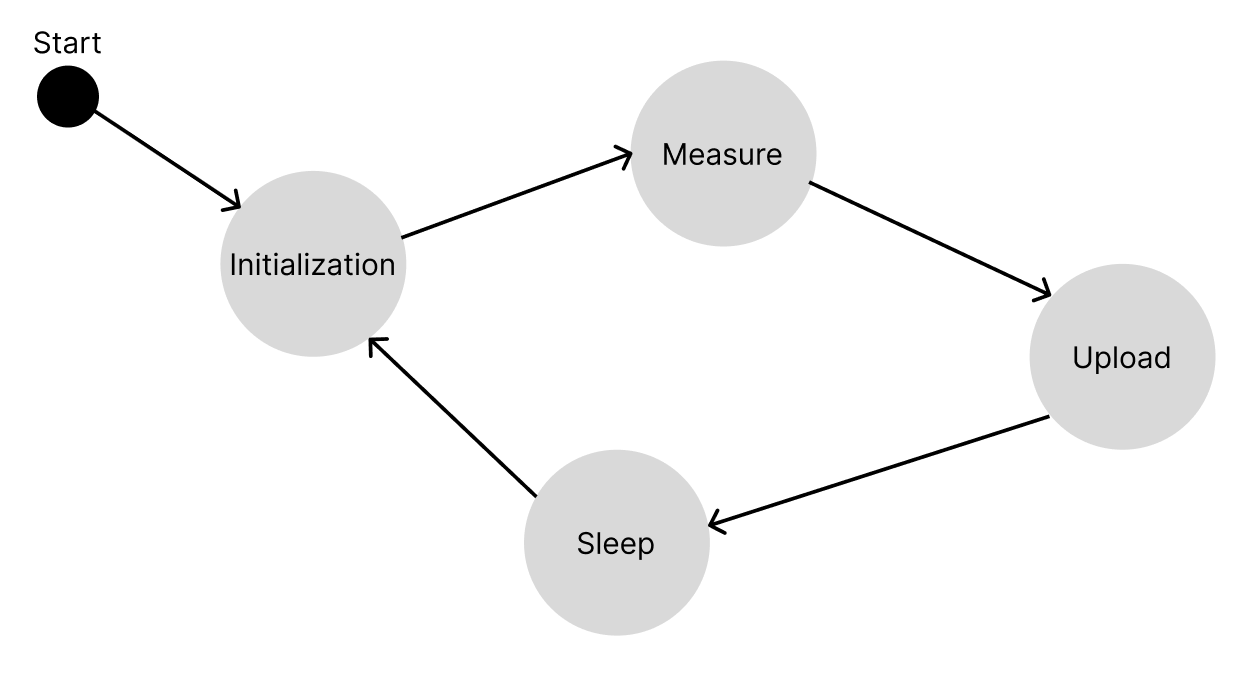
\includegraphics[width=\textwidth]{figures/KSA}
    \caption{Práca meteostanice vo forme konečno stavoho automatu. \label{ksa}}
\end{figure}

\subsection{Výsledok refaktorovania kódu.}
Takže na základe konečného stavového automatu zobrazeného na obrázku 1 som prepracoval štruktúru celého projektu. Nezmenený zostal len súbor \verb|helper.py|

Pre lepšie pochopenie novej štruktúry projektu najprv uvediem všetky súbory, ktoré sa v projekte nachádzajú: 
\begin{itemize}
    \item \verb|start.py| - štartovací súbor, ktorý obsahuje logiku prechodu z jedného stavu do druhého.
    \item \verb|states.py| - súbor, ktorý obsahuje celú logiku jednotlivých stavov.
    \item \verb|helper.py| - súbor s pomocnými funkciami.
    \item \verb|settings.py| - tu sa nachádzajú konštantné parametre, ktoré sa v projekte používajú na uľahčenie prístupu k nim.
\end{itemize}
Teraz sa pozrime na štruktúru projektu a jednotlivé súbory podrobnejšie.

Ako som povedal, poradie prechodu z jedného stavu do druhého sa nachádza v súbore \verb|start.py|, každý stav je obsiahnutý vo funkciách:
\begin{itemize}
    \item \verb|def init(context)| - inicializácia
    \item \verb|def measure(context)| - meranie
    \item \verb|def upload(context)| - nahrávanie
    \item \verb|def sleep_pico(context)| - uspávanie
\end{itemize}
Tieto funkcie sa nachádzajú v súbore \verb|states.py| a práve tieto funkcie budú musieť študenti naprogramovať. Okrem týchto funkcií môžu študenti vytvoriť aj iné funkcie, ale hlavné je, aby sa názov uvedených funkcií nemenil. Súbor \verb|start.py| obsahuje aj triedu \verb|Context|, ktorá sa používa ako globálna štruktúra s premennými. Tieto premenné sú pomocné a používajú sa v rôznych funkciách. Funkcie v súbore \verb|helper.py| nebudú študenti programovať a používajú sa skôr ako knižnicu. Súbor \verb|settings.py| obsahuje konfiguračné premenné, ktoré sa zvyčajne používajú len raz. Tieto premenné som oddelil do samostatného súboru, aby som zlepšil čistotu kódu a uľahčil zmenu týchto údajov.
%%------------------------------------------------------------------------

\section{Testovanie (Tretia iterácia)}
\subsection{Ciele}
Účelom testovania je skontrolovať, či projekt neobsahuje výrazné problémy alebo nejasnosti v návrhu projektu. Testovanie by sa malo vykonávať na cieľovej skupine projektu a malo by sa prednostne vzťahovať na celý projekt.

Ďalším účelom testovania je overenie množstva práce, ktorú študenti dokážu vykonať v stanovenom čase. Robí sa to preto, aby sa projekt dal ľahšie rozdeliť na niekoľko častí (prednášok). Je to preto, aby sa projekt ľahšie implementoval do kurzu.
\subsection{Príprava}
Test sa mal uskutočniť v Gymnáziume svätého Tomáša Akvinského\footnote{\textit{https://www.gta.sk/}}. Na test bola určená 1 hodina a 30 minút. Vo vymedzenom čase som chcel študentom odovzdať čo najviac informácií, preto som si pripravil podrobný plán postupu, aby sa minimalizovali časové straty.

Test som rozdelil na teoretickú a praktickú časť. V teoretickej časti som si dal za úlohu povedať o týchto veciach:
\begin{enumerate}
    \item Čo je to \gls{iot}.
    \item Porozprávať o vrstvách architektúry \gls{iot} riešení.
    \item Vysvetliť architektúru môjho projektu.
    \item Vyjadriť študentom, čo budú robiť v praktickej časti.
\end{enumerate}

Pri plánovaní praktickej časti som nemohol predpovedať, koľko práce budú študenti schopní urobiť v čase určenom na test. Preto som naplánoval pomerne veľa položiek, a to:

\begin{enumerate}
    \item Poskladanie hardvérovej časti projektu.
    \item Testovanie blikaním \textit{\gls{led}} diódy.
    \item Meranie hodnôt zo senzorov.
    \item Pripojenie k internetu a \gls{mqtt} brokeru.
    \item Odosielanie údajov vo formáte \gls{json}.
    \item Implementácia zníženia spotreby energie.
    \item Signalizácia problémov pomocou \textit{\gls{led}} diódy.
    \item Zápis a čítanie údajov zo súboru.
\end{enumerate}

Praktická časť bola implementovaná na doskách \textit{ESP32}, pretože škola mala k dispozícii len ich. S ohľadom na to som upravil schému pripojenia k doske. 

Na programovanie som sa rozhodol použiť \textit{\gls{ide} Thoony}, pretože už bolo nainštalované na školských počítačoch.

Pri príprave a realizácii testu mi pomáhal Šimon Pavlišin a ja som bol vedúcim testu.

\subsection{Úroveň znalostí študentov}

Test bol realizovaný na študentoch tretieho ročníka Gymnázia svätého Tomáša Akvinského. V čase testovania študenti už mali za sebou praktické úlohy s \textit{Arduino Uno} a \textit{ESP32}. Mali teda základné zručnosti v programovaní mikroelektroniky. Takéto schopnosti mohli zrýchliť niektoré fázy praktickej časti (napr. pripojenie modulov k doske \textit{ESP32}).

\subsection{Výsledky}

Na teste sa zúčastnilo 12 študentov s rôznou úrovňou motivácie a znalostí. Počas testu sa mi podarilo spracovať celú teoretickú časť a prvé dva body praktickej časti.  Študenti mali problémy s poskladaním hardvéru a mali veľké problémy s pochopením \textit{Thonny}, takže veľa času sme venovali riešeniu problémov súvisiacich s týmto \gls{ide}.

Podľa študentov bola teoretická časť pomerne ľahko pochopiteľná, ale praktická časť bola dosť nejasná.

\subsection{Záver}

Tento test umožnil získať veľa užitočných informácií a pomohol vyhnúť sa niektorým problémom pri písaní scenára pre lekcie. 

Fakt toho, že títo študenti už mali hodiny s \textit{ESP32}, im nedal výraznú výhodu, pretože moduly k \textit{EP32} pripojovali dosť dlho. Prekvapilo ma množstvo času stráveného riešením kritických problémov s \textit{\gls{ide} Thonny}. Študenti nechápali, ako ho používať, a robili veľmi jednoduché chyby, ale ich riešenie mi zabralo dosť času. Myslím si, že tento problém vznikol v dôsledku môjho zlého plánovania, pretože som predpokladal, že táto fáza nezaberie veľa času, a tak som jej nevenoval dostatočnú pozornosť. Túto skúsenosť zohľadním pri príprave svojich hodín.

Vo všeobecnosti mi tento test poskytol predstavu o približnom množstve informácií, ktoré musím poskytnúť na jednej vyučovacej hodine môjho kurzu. Poskytol mi tiež neoceniteľné skúsenosti pri práci so študentmi.

\section{Zhromažďovanie údajov na bráne a ich spracovanie}

Po ukončení vývoja meteorologickej stanice považujem za účelné ukázať študentom, ako pracovať so získanými údajmi, spracovať ich a vizualizovať. 

Ako už bolo popísané v teoretickej časti, najlepšie sa to robí pomocou programovacieho jazyka \textit{Node Red} na pripravenej \gls{iot} bráne. Vytvoril som teda pomerne jednoduchý program (obr. \ref{node}) na vizualizáciu údajov získaných z meteorologickej stanice. Jeho vizualizáciu si môžete pozrieť na obrázku \ref{nodeVisual}.
\begin{figure}[!ht]
    \centering
    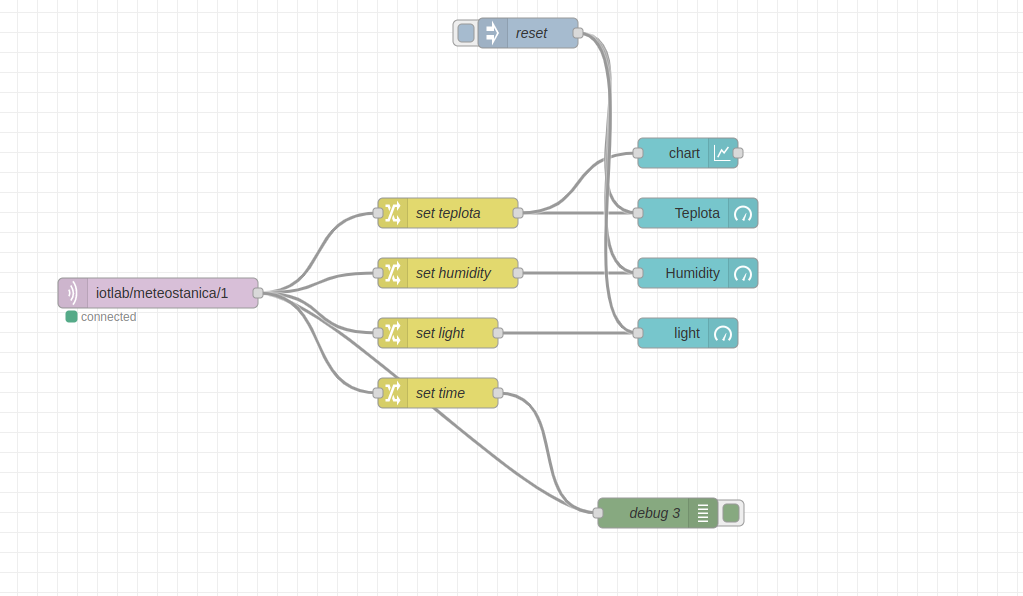
\includegraphics[width=\textwidth]{figures/node}
    \caption{Logika aplikácie na vizualizáciu dát vytvorenej v \textit{Node Red} \label{node}}
\end{figure}
\begin{figure}[!ht]
    \centering
    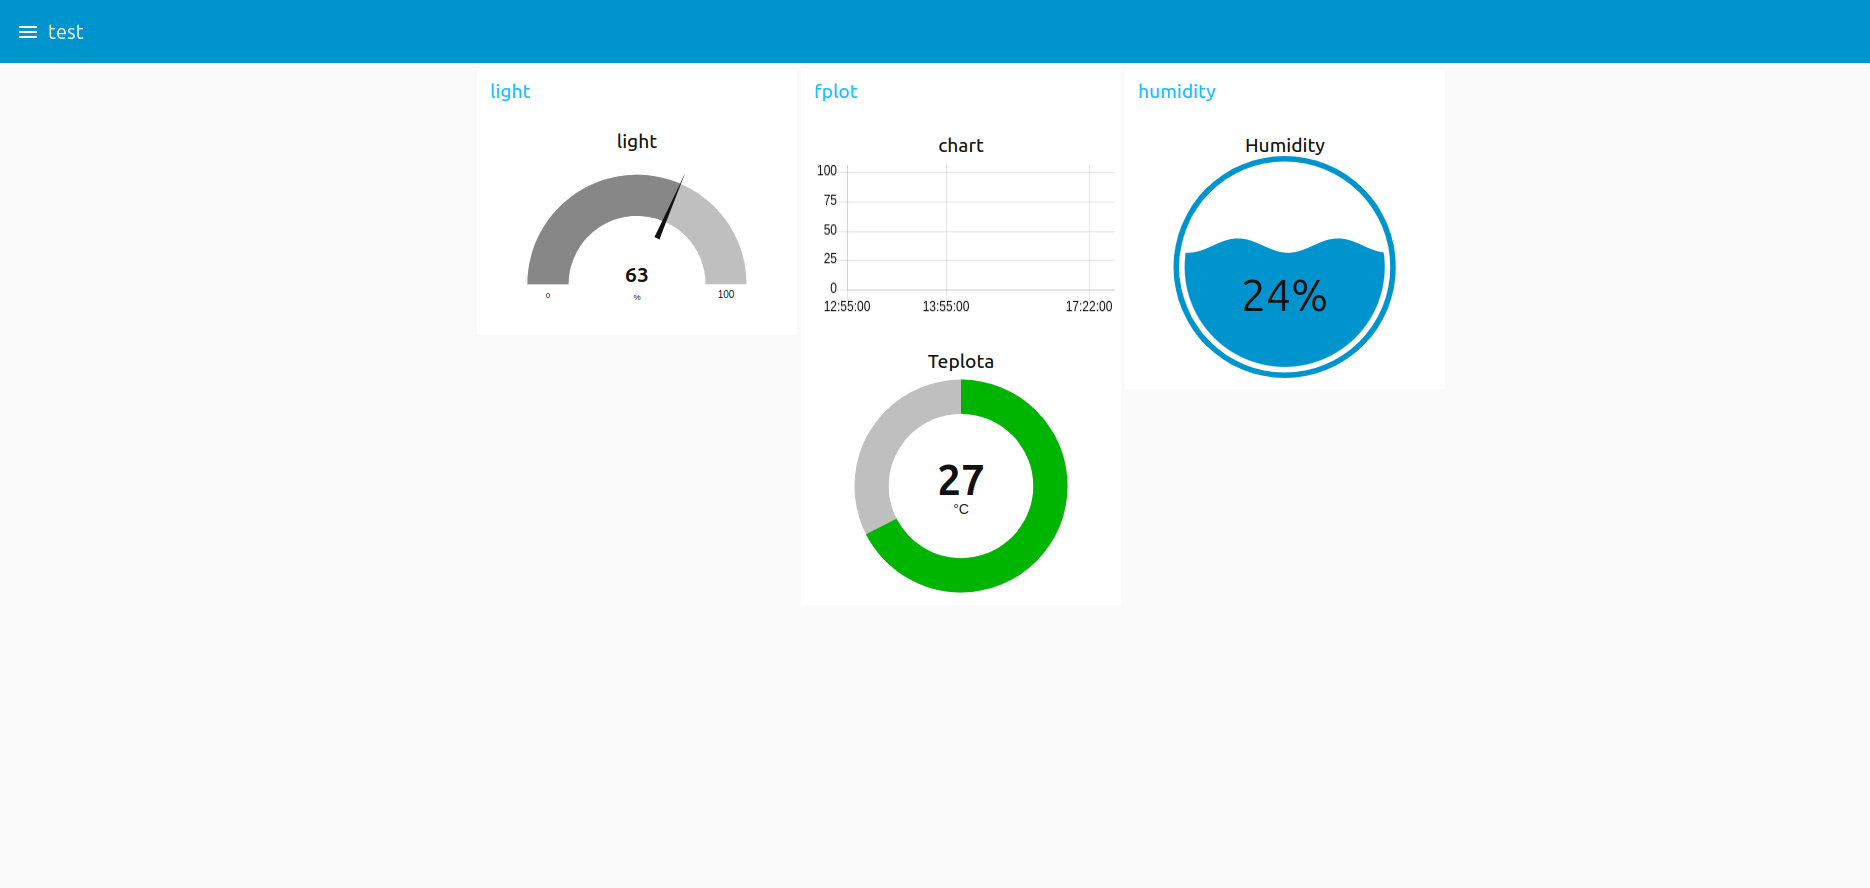
\includegraphics[width=\textwidth]{figures/node_obr}
    \caption{Vizualizácia aplikácie vytvorenej na \textit{Node Red}. \label{nodeVisual}}
\end{figure}
Napriek tomu, že logika programu je veľmi jednoduchá, na základe mojich skúseností môžem povedať, že na bežné zoznámenie s jazykom \textit{Node Red} tohto stačí. 

Program na obrázku \ref{node} je len príkladom. Učitelia si pri implementácii môjho projektu do svojho kurzu môže vytvoriť vlastný scenár na základe vedomostí svojich študentov.

\section{Analiza pridanej hodnoty projektu}
\subsection{Hlavná časť analýzy}
Táto časť opisuje cenu niekoľkých projektových konfigurácií, a konkrétne:
\begin{enumerate}
    \item Pomocou \textit{Raspberry Pi Pico WH} (obrázok \ref{f_pico}).
    \item Pomocou \textit{Raspberry Pi Pico WH} s použitím \textit{Cytron Maker Pi Pico Base W} (obrázok \ref{f_b_pico}).
    \item Pomocou \textit{ESP32} (obrázok \ref{f_esp32}). 
\end{enumerate}
Ceny som prebral z webovej stránky \textit{rpishop.cz}, pretože si myslím, že tam uvedené ceny plne zodpovedajú cenám na trhu. Okrem toho som analyzoval ceny na stránke \textit{aliexpress.com}, aby som zobraziť, potenciálne, najnižšie možné ceny. 

Treba poznamenať, že v čase písania tejto práce ešte neboli odstránené škodlivé následky krízy mikročipov\footnote{\textit{https://www.telefonica.com/en/communication-room/why-is-the-microchip-crisis-affecting-us-this-much/}}, takže cenová politika sa môže za nejaký čas výrazne zmeniť.  

Ako už bolo spomenuté v iných kapitolách, stredné školy na Slovensku už zvyčajne majú k dispozícii stavebnice Arduino Kit, ktoré obsahujú moduly potrebné na kurz: \gls{dht}, \gls{ldr}, \gls{led} diódy. Preto som sa rozhodol ich cenu do kalkulácie nezahŕňať. Pre \gls{gw} som sa rozhodol použiť \textit{Raspberry Pi 3 Model A+}, pretože tento model je dostatočne výkonný na svoje úlohy.

Všetky výpočty sú k dispozícii v tabuľkách \ref{tabESP32}, \ref{tabPico} a \ref{tabPicoDos}. Výpočty boli vykonané v mene Euro(\texteuro).

\begin{table}[!ht]
    \smallskip
    \centering
    \begin{tabular}{ | m{3cm} | m{2cm}| m{2cm} | m{2cm} | m{3cm} | } 
        \hline
         & \textit{ESP32} & \textit{Raspberry Pi 3 Model A+} & Celková cena & Cena projektu pre 30 študentov\\
        \hline
        rpishop.cz & 10,81 \texteuro & 33,88 \texteuro & 44,69 \texteuro & 358,18 \texteuro\\
        \hline
        aliexpress.com & 6,67 \texteuro & 85,43 \texteuro & 92,10 \texteuro & 285,53 \texteuro\\
        \hline
    \end{tabular}    
    \smallskip
    \caption{Analýza ceny projektu na základe dosky \textit{ESP32}. \label{tabESP32}}
\end{table}


\begin{table}[!ht]
    \smallskip
    \centering
    \begin{tabular}{ | m{3cm} | m{2cm} | m{2cm} | m{2cm} | m{3cm} | } 
        \hline
         & \textit{Raspberry Pi Pico WH} & \textit{Raspberry Pi 3 Model A+} & Celková cena & Cena projektu pre 30 študentov\\
        \hline
        rpishop.cz & 8,86 \texteuro & 33,88 \texteuro & 42,74 \texteuro & 308,54 \texteuro\\
        \hline
        aliexpress.com & 5,83 \texteuro & 85,43 \texteuro & 91,26 \texteuro & 260,33 \texteuro\\
        \hline
    \end{tabular}    
    \smallskip
    \caption{Analýza ceny projektu na základe dosky \textit{Raspberry Pi Pico WH}. \label{tabPico}}
\end{table}


\begin{table}[!ht]
    \smallskip
    \centering
    \begin{tabular}{ | m{7em} | m{4em} | m{4em} | m{2cm} | m{4em} | m{5em} | } 
        \hline
         & \textit{Raspberry Pi Pico WH} & \textit{Cytron Maker Pi Pico Base W} & \textit{Raspberry Pi 3 Model A+} & Celková cena & Cena projektu pre 30 študentov\\
        \hline
        rpishop.cz & 8,86 \texteuro & 11,02 & 33,88 \texteuro & 42,74 \texteuro & 308,54 \texteuro\\
        \hline
        aliexpress.com & 5,83 \texteuro & - & 85,43 \texteuro & - & -\\
        \hline
    \end{tabular}    
    \smallskip
    \caption{Analýza ceny projektu na základe dosky \textit{Raspberry Pi Pico WH} a \textit{Cytron Maker Pi Pico Base W}. \label{tabPicoDos}}
\end{table}

\subsection{Záver analýzy}

Vzhľadom na vyššie uvedené výpočty môžeme povedať, že pri nákupe komponentov z \textit{aliexpress.com} nebudú úplne lacnejšie ako v iných internetových obchodoch mikroelektroniky.  Ak sa projekt bude vyvíjať na základe dosky \textit{ESP32}, potom bude lacnejšie kúpiť ich na aliexpress.com, ale musíte brať do úvahy kvalitu tohto výrobku. Pri analýze ceny som na stránke \textit{aliexpress.com} nenašiel dosku \textit{Cytron Maker Pi Pico Base W}, takže ak sa rozhodnete pre túto konfiguráciu, musíte si toto zariadenie kúpiť na iných stránkach.

% !TEX root = ../thesis.tex

\chapter{Vyhodnotenie}
\label{evaluation}

V tejto časti podrobne opíšem projekt, ktorý sa podarilo zrealizovať. Zanalyzujem jeho plusy a mínusy. Uvediem aj možné alternatívne riešenia alebo doplnenia existujúceho projektu.

\section{Téma a architektúra projektu}

Vypracoval som systém zberu meteorologických dát (obr. \ref{proekt}), ktorý zahŕňa 3 úrovne architektúry \gls{iot} (obr. \ref{iot}). 

Počas plánovania a vývoja projektu bola otázka výberu témy pomerne diskutabilná, pretože výber témy priamo súvisí s architektúrou projektu a jeho obsahom. Obával som sa, že projekt bude drahší a príliš komplikovaný, preto som do projektu zapojil len senzory. Chápal som tiež, že je dôležité ukázať študentom niekoľko úrovní architektúry internetu vecí, preto som sa rozhodol pridať do projektu IoT bránu. 

Výber hlavného inteligentného zariadenia pre meteorologickú stanicu bol tiež dosť diskutabilný. Veď najlacnejšou možnosťou by bolo \textit{Arduino Uno}, ale ja som vybral \textit{Raspberry Pi Pico W} z viacerých dôvodov opísaných v osobitnej časti. 

Ak projekt posúdite z hľadiska externého, môžete dospieť k záveru, že jeho komponenty možno nahradiť lacnejšími alebo energeticky úspornejšími. Pri vývoji tohto projektu som však chcel vytvoriť platformu na učenie, nie priemyselný výrobok. Preto som väčšinu svojich rozhodnutí robil z hľadiska práce so študentmi.

Verím, že architektúra môjho riešenia je racionálne vyvážená a dobre premyslená.

\section{Softvér meteostanice}
Architektúra softvéru meteostanice je založená na 4 fyzikálnych stavoch jeho životného cyklu (obr. \ref{ksa}). Jednotlivé funkcie softvéru sú rozdelené medzi týmito stavmi. Softvér obsahuje základné funkcie IoT riešenia. Na programovanie meteostanice sa použil programovací jazyk \textit{Micropython}. 

Pre prípadných študentov, ktorí by tento projekt vyvíjali, som vytvoril kostru programu. Preto plne naprogramovaný projekt slúži len ako príklad pre učiteľa.

Myslím si, že architektúra kódu je dokonalá, ale napĺňanie funkcií jednotlivých stavov sa ukázalo ako dosť chaotické a neprehľadné. Preto by som neodporúčal, aby študenti presne reprodukovali môj kód.

\section{Program na bráne}

Projekt má bránu \gls{mqtt}, ktorá zhromažďuje všetky údaje odoslané z meteorologických staníc a zobrazuje ich na webovom rozhraní. Návrh brány bol prevzatý z bakalárskej práce \textit{Šimona Pavlišina}\cite{bookSimon}. Programovací jazyk použitý v tejto fáze je \textit{Node Red}.

Môžem povedať, že program, ktorý som napísal, je pomerne jednoduchý. Je to spôsobené tým, že som nechcel túto etapu komplikovať, ale prvýkrát sa zoznámiť s jazykom \textit{Node Red} a z mojich skúseností môžem povedať, že takéto ľahké programy sú na túto úlohu ako stvorené.

V prípade potreby môže učiteľ na základe znalostí svojich študentov a dostupných údajov vymyslieť iný scenár.

\section{Testovanie}

Projekt bol testovaný na reálnych študentoch stredných škôl. Testovanie sa uskutočnilo na študentoch \textit{Gymnázia svätého Tomáša Akvinského} na 12 člennej skupine a trvalo 1 hodinu a 30 minút. Cieľom testovania bolo overiť možnosť implementácie môjho projektu do vzdelávacieho kurzu v praxi a overiť, na koľko približných častí by sa mal projekt rozdeliť, aby sa dal preniesť do kurzu.

Výsledkom testovania bolo, že v projekte neboli zistené žiadne kritické problémy. Po testovaní sa ukázalo, že tento projekt by sa mohol rozdeliť na 4 - 5 častí pre implementáciu do kurzu.

Žiaľ, vzhľadom na mnohé okolnosti som nemohol projekt otestovať v plnom rozsahu a myslím si, že to je dosť veľké pochybenie tejto práce. Veď na objektívne posúdenie tejto práce je potrebné mať dobre otestovaný produkt.

\section{Zhrnutie}

Myslím si, že táto práca je celkom dobrá, ale ešte sa dá teoreticky rozvinúť. Podľa môjho názoru je téma vzdelávacích projektov veľmi široká, takže tento projekt môže byť začiatkom niečoho nového.


% !TEX root = ../thesis.tex

\chapter{Záver}
\label{summary}

V tejto bakalárskej práci som analyzoval existujúce edukačné projekty pre študentov stredných škôl zamerané na propagáciu \gls{iot} a spoznávanie jeho základných funkcií.  

Na základe tejto analýzy som naplánoval a vypracoval projekt s architektúrou \gls{iot} zameraný na jeho implementáciu do učebného kurzu stredných škôl na Slovensku.

Projekt obsahuje základné funkcie typických riešení \gls{iot} (pripojenie na internet, sledovanie času, odosielanie údajov na server atď.) Pre jednoduchšiu implementáciu do vzdelávacieho kurzu som pre študentov vytvoril kostru projektu. 

Projekt bol otestovaný na vzorke 12 študentov. Napriek tomu, že táto skupina je pomerne malá a projekt nebol úplne rozpracovaný, umožnilo to pochopiť niektoré jeho hlavné nedostatky a pomôže vyhnúť sa ďalším ťažkostiam pri implementácii projektu v kurze.

K projektu bola vytvorená podrobná dokumentácia.

% good linebraking of bibtex url
\setcounter{biburllcpenalty}{7000}
\setcounter{biburlucpenalty}{8000}

%% The bibliography
\printbibliography[heading=bibintoc]

\label{theend} % the last page of the thesis

% List of acronyms
\printglossary[type=\acronymtype,title={\acrlistname}]

% Glossaries
\printglossary

%% Appendix
% !TEX root = ../thesis.tex

\chapter*{\appendixlistname}
\addcontentsline{toc}{chapter}{\appendixlistname}

\begin{description}
	\item[\appendixname{} A] Štruktúra projektu
\end{description}

\appendix
\renewcommand\chaptername{\appendixname}
% !TEX root = ../thesis.tex

\chapter{Štruktúra projektu}
Z hardvérového hľadiska sa projekt skladá z dvoch častí:

\begin{itemize}
    \item Meteostanice - zbierajú údaje z prostredia a prenášajú ich do \gls{gw}. Túto časť vyvíjajú študenti. Každý jednotlivý študent si vyvíja vlastnú meteorologickú stanicu, preto je potrebné pri plánovaní kurzu zabezpečiť, aby boli všetky potrebné moduly pre meteorologické stanice k dispozícii v dostatočnom množstve.
    \item \gls{iot} \gls{gw} - zariadenie, ktoré sa používa na zhromažďovanie informácií zo všetkých meteorologických staníc jednej študijnej skupiny. Prevádzku tohto zariadenia je potrebné nakonfigurovať pred začatím štúdia študentov.
\end{itemize}

\section{Súčasti meteostanice}
\subsection{Hardvér meteostanice}
Hardvér meteostanice pozostáva z:
\begin{itemize}
    \item \textit{Raspberry Pi Pico W} - hlavné inteligentné zariadenie, ktorého logiku musia naprogramovať študenti.
    \item \gls{ldr} - senzor na meranie osvetlenia.
    \item \gls{dht} je senzor na meranie vlhkosti a teploty.
    \item \gls{led} dióda - slúži na signalizáciu problémov.
\end{itemize}
Všetky komponenty meteorologickej stanice sú pripojené k doske Raspberry Pi Pico W pomocou káblov, schéma zapojenia je znázornená na obrázku \ref{schema1}. Na zjednodušenie pripojenia môžete použiť pomocnú dosku Cytron \textit{Maker Pi Pico Base W}.

\begin{figure}[!ht]
    \centering
    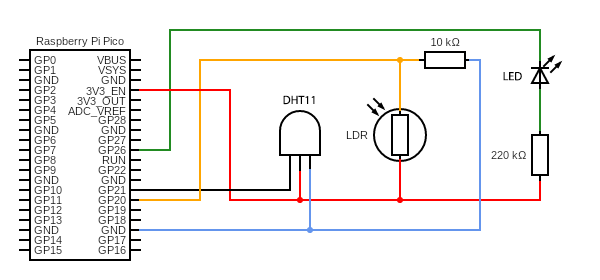
\includegraphics[width=\textwidth]{figures/circuit}
    \caption{Chéma pripojenia k doske Raspberry pi pico W \label{schema1}}
\end{figure}

V prípade potreby možno dosku \textit{Raspberry Pi Pico W} zameniť na dosku \textit{ESP32}. Teoreticky by s použitím tejto dosky nemali byť žiadne problémy, ale táto verzia nebola úplne otestovaná.

\subsection{Softvér meteostanice}
Celá logika meteostanice je napísaná v programovacom jazyku \textit{MicroPython} verzie v1.20.0. 

Program projektu sa skladá z niekoľkých súborov:
\begin{itemize}
    \item \verb|start.py| - štartovací súbor celého programu, ktorý obsahuje logiku prechodu z jedného stavu do druhého.
    \item \verb|states.py| - súbor, ktorý obsahuje logiku jednotlivých stavov. 
    \item \verb|helper.py| - pomocné funkcie. 
    \item \verb|settings.py| - súbor pre systémové premenné. 
    \item \verb|data.txt| - súbor vyrovnávacej pamäte na ukladanie neodoslaných údajov.
\end{itemize}
Projekt používa aj knižnicu tretej strany s názvom \verb|umqtt.simple| na pripojenie k \gls{mqtt} brokeru. 

Životný cyklus meteostanice pozostáva zo 4 stavov a je popísaný funkciami v kóde aplikácie.

Konkrétne funkcie:

\begin{itemize}
    \item \verb|init| - v tejto funkcii sa zariadenie pripojí k \textit{WiFi} a \gls{mqtt} a synchronizuje čas. Úspešnosť pripojenia je signalizovaná prostredníctvom \gls{led} diódy. 
    \item \verb|measure| - zariadenie meria vlhkosť, teplotu, úroveň svetla a čas merania. Potom sa údaje prevedú do formátu JSON na ďalší export.
    \item \verb|upload| - zozbierané údaje sa odošlú do \gls{mqtt} brokera. Ak sa zariadenie nemohlo pripojiť k sieti WiFi alebo k brokeru \gls{mqtt}, údaje sa archivujú do súboru data.txt a odošlú sa pri ďalších pokusoch na pripojenie k internetu. 
    \item \verb|sleep_pico| - zariadenie sa prepne do energeticky efektívneho režimu na pridelený čas.
\end{itemize}

Počas školenia študenti dostanú tieto funkcie prázdne a ich úlohou je naprogramovať vyššie uvedenú logiku v rámci týchto funkcií. Učiteľ počas programovania vystupuje ako supervízor a mentor.

\section{Súčasti \gls{iot} brány}
\subsection{Hardvér}
\gls{gw} sa skladá len z jednej časti, konkrétne z mikropočítača \textit{Raspberry Pi 3}. Môžete použiť aj novšiu verziu, konkrétne \textit{Raspberry Pi 4}. 

Zariadenie musí byť pripojené k internetu prostredníctvom káblového pripojenia alebo cez adaptér \textit{WiFi}. 

\subsection{Softvér}
\gls{gw} je založený na technológii Mosquito a má nainštalovaný Docker a \textit{Node Red}. Podrobnejšiu konfiguráciu systému nájdete v bakalárskej práci \textit{Otvorený \gls{iot} Lab pre stredné školy}\cite{bookSimon}. 

V tejto fáze vývoja projektu študenti používajú programovací jazyk \textit{Node Red} na analýzu a vizualizáciu údajov odosielaných z meteorologickej stanice. Na obrázku \ref{nodeVisual1} je znázornený príklad takejto vizualizácie.

\begin{figure}[!ht]
    \centering
    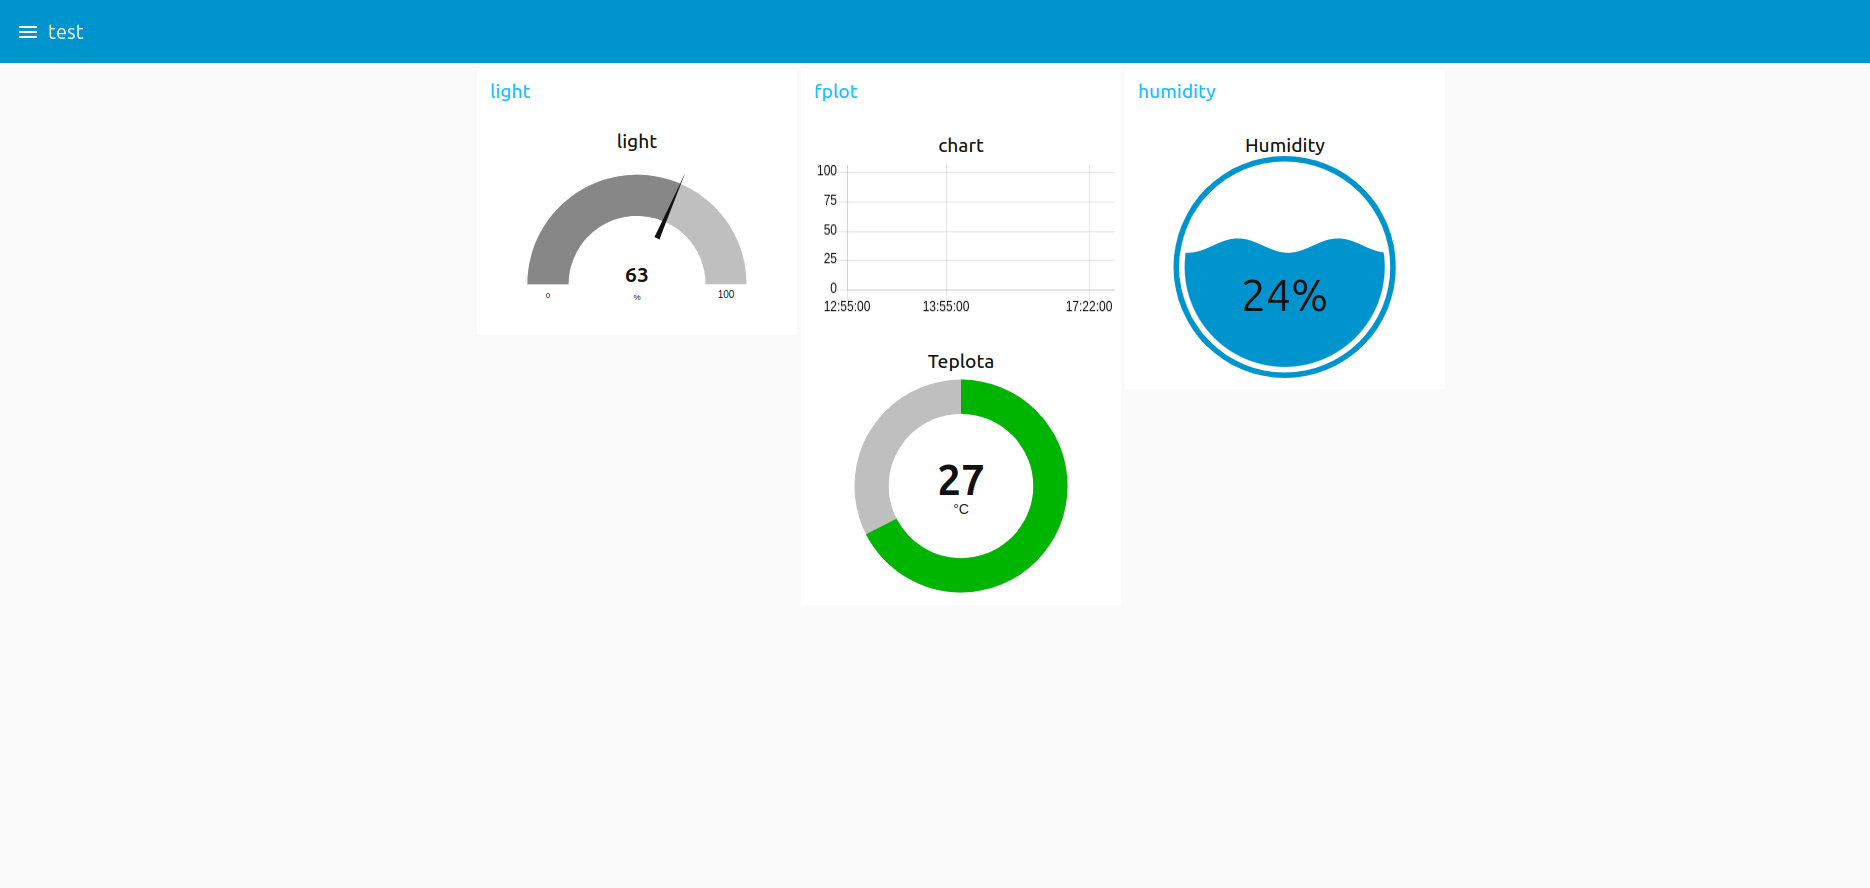
\includegraphics[width=\textwidth]{figures/node_obr}
    \caption{Vizualizácia aplikácie vytvorenej na \textit{Node Red}. \label{nodeVisual1}}
\end{figure}

\subsection{Alternatívny postup}
Vo všeobecnosti môže ako brána slúžiť akýkoľvek iný počítač (napr. počítač učiteľa), pokiaľ je na ňom nakonfigurovaný \gls{mqtt} broker (napr. \textit{Hivemq} alebo \textit{Mosquito}) a nainštalovaný \textit{Docker} a \textit{Node Red}.


% zivotopis autora
%\curriculumvitae\protect
%Táto časť\/ je nepovinná. Autor tu môže uviesť\/ svoje biografické
%údaje, údaje o~záujmoch, účasti na~projektoch, účasti na~súťažiach,
%získané ocenenia, zahraničné pobyty na~praxi, domácu prax, publikácie
%a~pod.

\end{document}
